\chapter{高輝度LHC-ATLAS実験に向けたエンドキャップミューオントリガーの統合}
\label{chap_TriggerIntegration}

\section{トリガー開発の流れとこれまでの性能検証}
\label{sec_TriggerTestSystem}
本節では、これまでのトリガーロジック開発フローを説明し、本研究で取り組んだ実機試験の位置付けを明らかにする。図\ref{Develop_flow}にトリガーロジックの開発フローを示す。トリガーの開発はまず高輝度LHC-ATLAS実験におけるL0 Trigger systemの要求 (トリガー効率、再構成した角度分解能、トリガーレート、トリガーレイテンシー) を満たすよう、前章で紹介したコンセプトが設計された。次にそのコンセプトをデジタル回路上で実現される論理回路として実装するため、モジュールごとにHDL開発が行われた。HDLで書かれたファームウェアはVivadoによるインプリメンテーション\footnote{Vivadoのインプリメンテーションプロセスは、主に1. ロジック最適化、2.デザイン配置、3.配置後のデザインの物理最適化、4. デザインの配線、5. 配線後のデザインの物理最適化、6 ビットストリームの生成で構成される。}を経て、ハードウェアで動作させることができる。また、それぞれの工程において検証システムも同時に整備されており、開発とフィードバックのループを回すことで、期待した性能をもつトリガーが実現できていることを確かめながら、着実に開発を進めている。

\begin{figure} 
\centering
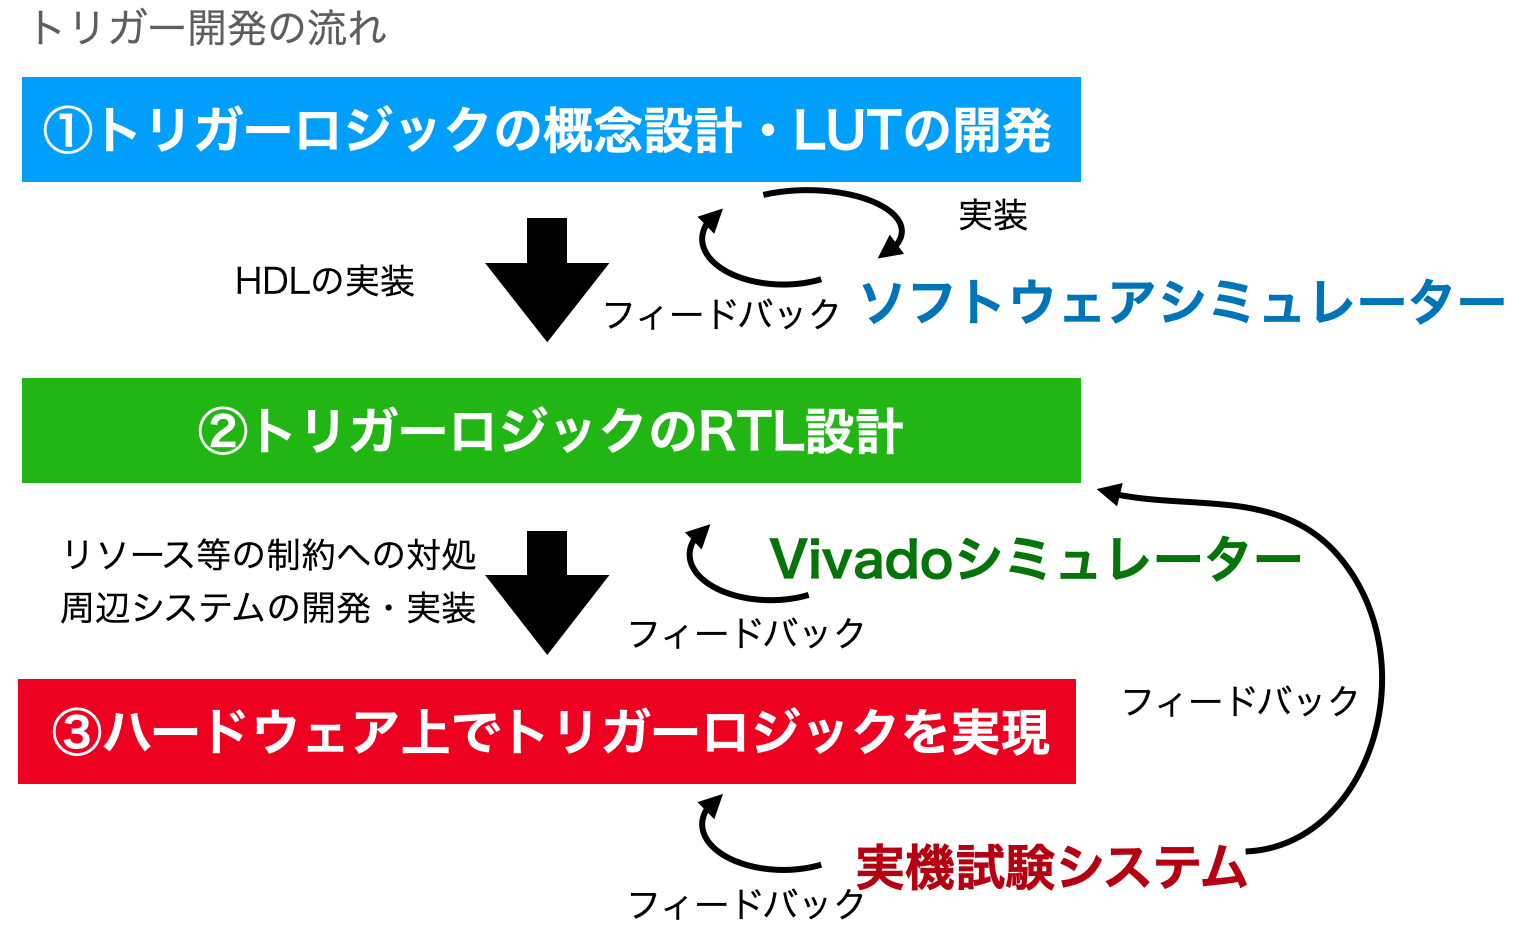
\includegraphics[width=16cm]{fig/Test/Develop_flow.png}
\caption[TGCトリガー開発の流れ]{TGCトリガー開発の流れ。}
\label{Develop_flow}
\end{figure}

\subsection*{トリガーロジックの概念設計}
設計されたロジックの概念を、より具体的なデザインに落とし込み、その性能を評価する作業にはソフトウェアシミュレーターが用いられた。ソフトウェアは開発が容易で、ロジックの実装→性能評価→ロジックの修正→…という開発サイクルを比較的早く回すことができる。そのため、グローバルなデザインを決めていく初期の開発では重宝された。例えば、TGC BW 7層のヒット情報をStatino Coincidenceにより3つの代表点に絞り、その後パターンマッチングで角度情報を取得する、などの大枠の設計はここで決められた。また、各コインシデンスロジックの最小単位であるユニットの定義や、Segment Reconstructionで複数の飛跡候補が存在する時に、ヒットレイヤーの多さを基準に候補を絞る、などの具体的なデザインもここで決められた。さらに、パターンマッチングに利用されるLUTもロジックの設計と同時にソフトウェア的に開発されており、ソフトウェアシミュレーターはLUTも含めたトリガーロジックの性能評価を行っている。

図\ref{Soft_WS}にソフトウェアシミュレーターで測定された、TGC BW コインシデンスのトリガー効率を示す。トリガー効率の評価にはSingle Muon MCサンプルが用いられた。このイベントにはフォワードおよびエンドキャップ領域 ($1.05 < | \eta | < 2.4$) 、$\phi$全領域 (-3.14 < $\phi$ < 3.14) が含まれる。MCサンプルに含まれるTGC チェンバーのヒットチャンネル情報をトリガーロジックのインプットとして利用している。Efficiencyは以下のように定義され\pt 閾値ごとにビンわけされている。

\begin{equation}
\mathrm{Efficiency} = \frac{\mathrm{TGC\,BW\,coincidenceで}\,p_{\mathrm{T}}\,閾値20、15、10、5\,\mathrm{GeV}と判断されたミューオンの数}{オフラインで再構成されたミューオンの数}
\end{equation}

プラトー領域でのEfficiencyは94 \%程度で、高い検出効率を貯まっている。また閾値より低い\pt のミューオンを効率的に削減することができている。

\begin{figure} 
\centering
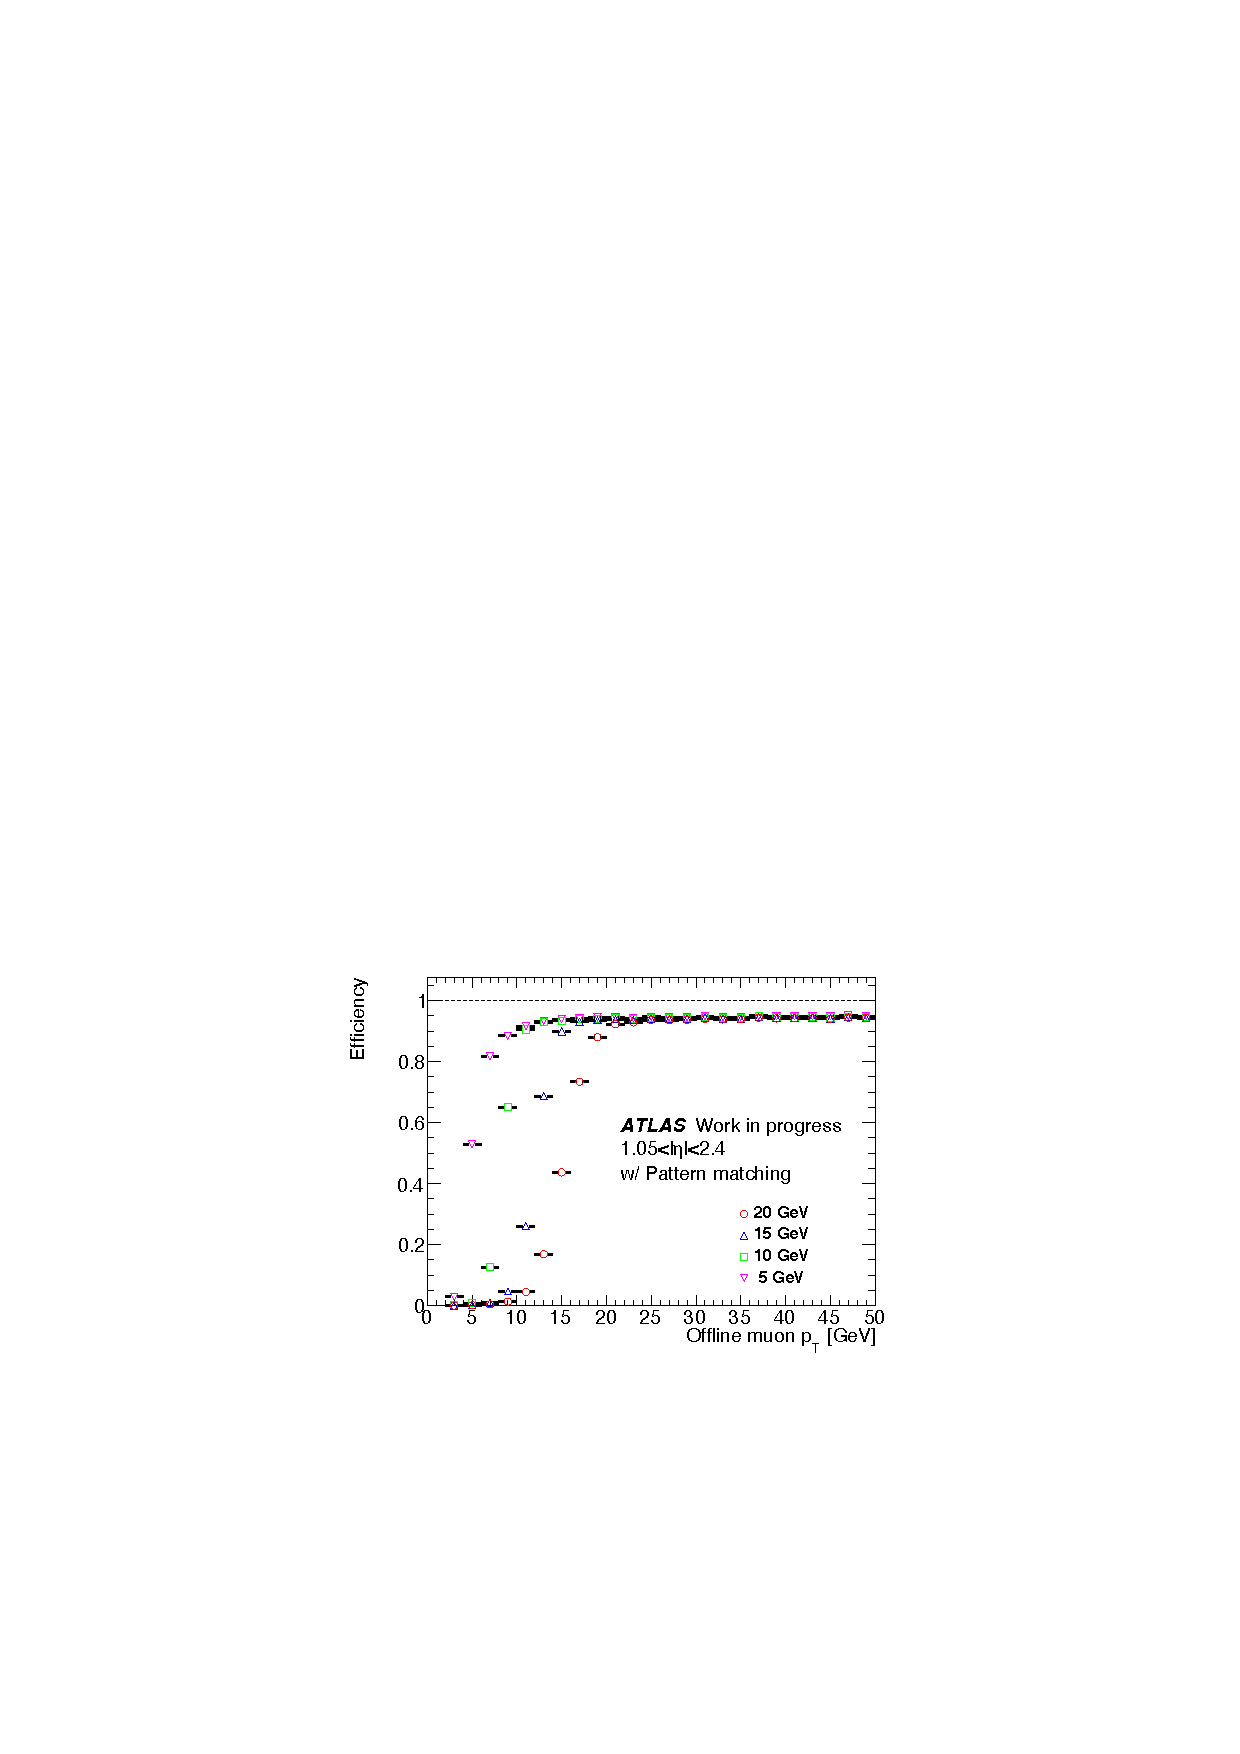
\includegraphics[width=16cm]{fig/Test/Soft_WS.pdf}
\caption[ソフトウェアシミュレーターで測定された、Wire Strip Coincidenceのトリガー効率]{ソフトウェアシミュレーターで測定された、Wire Strip Coincidenceのトリガー効率\cite{SLPDR}}
\label{Soft_WS}
\end{figure}

\subsection*{トリガーロジックのRTL実装}
次に開発されたロジックを実現するRegister Transfer Level (RTL) の設計が進められた。この過程ではソフトウェアで記述された論理を、Hardware Description Language (HDL) と呼ばれるデジタル回路における信号遷移におとしこむ作業が行われた。開発されたRTLの動作検証および実装されたトリガー回路の性能評価には、Vivado シミュレーターが用いられる。Vivado シミュレーターとはHDLで記述されるデジタル回路の動作をエミュレートするソフトウェアツールで、ロジック全体の信号の遷移を厳密にシミュレーションし、任意の信号をプローブすることができる。

Vivado シミュレーターで行われた各モジュールの性能評価の結果を述べる。Wire Segment Reconstructionの性能評価の結果を図\ref{Vivado_Wire_Efficiency}に示す。この試験でも同様のSingle Muon MCサンプルが利用され、イベント数は150,000 である。MCサンプルに含まれるTGC チェンバーのヒットチャンネル情報をWire Station Coincidenceのインプットに適したフォーマットに整形し、それに対する応答を調査しているEfficiencyは以下のように定義され、Truth Muonの$\eta$、$\phi$ごとにビンわけされている。

\begin{figure}
\begin{minipage}[b]{.5\linewidth}
\centering
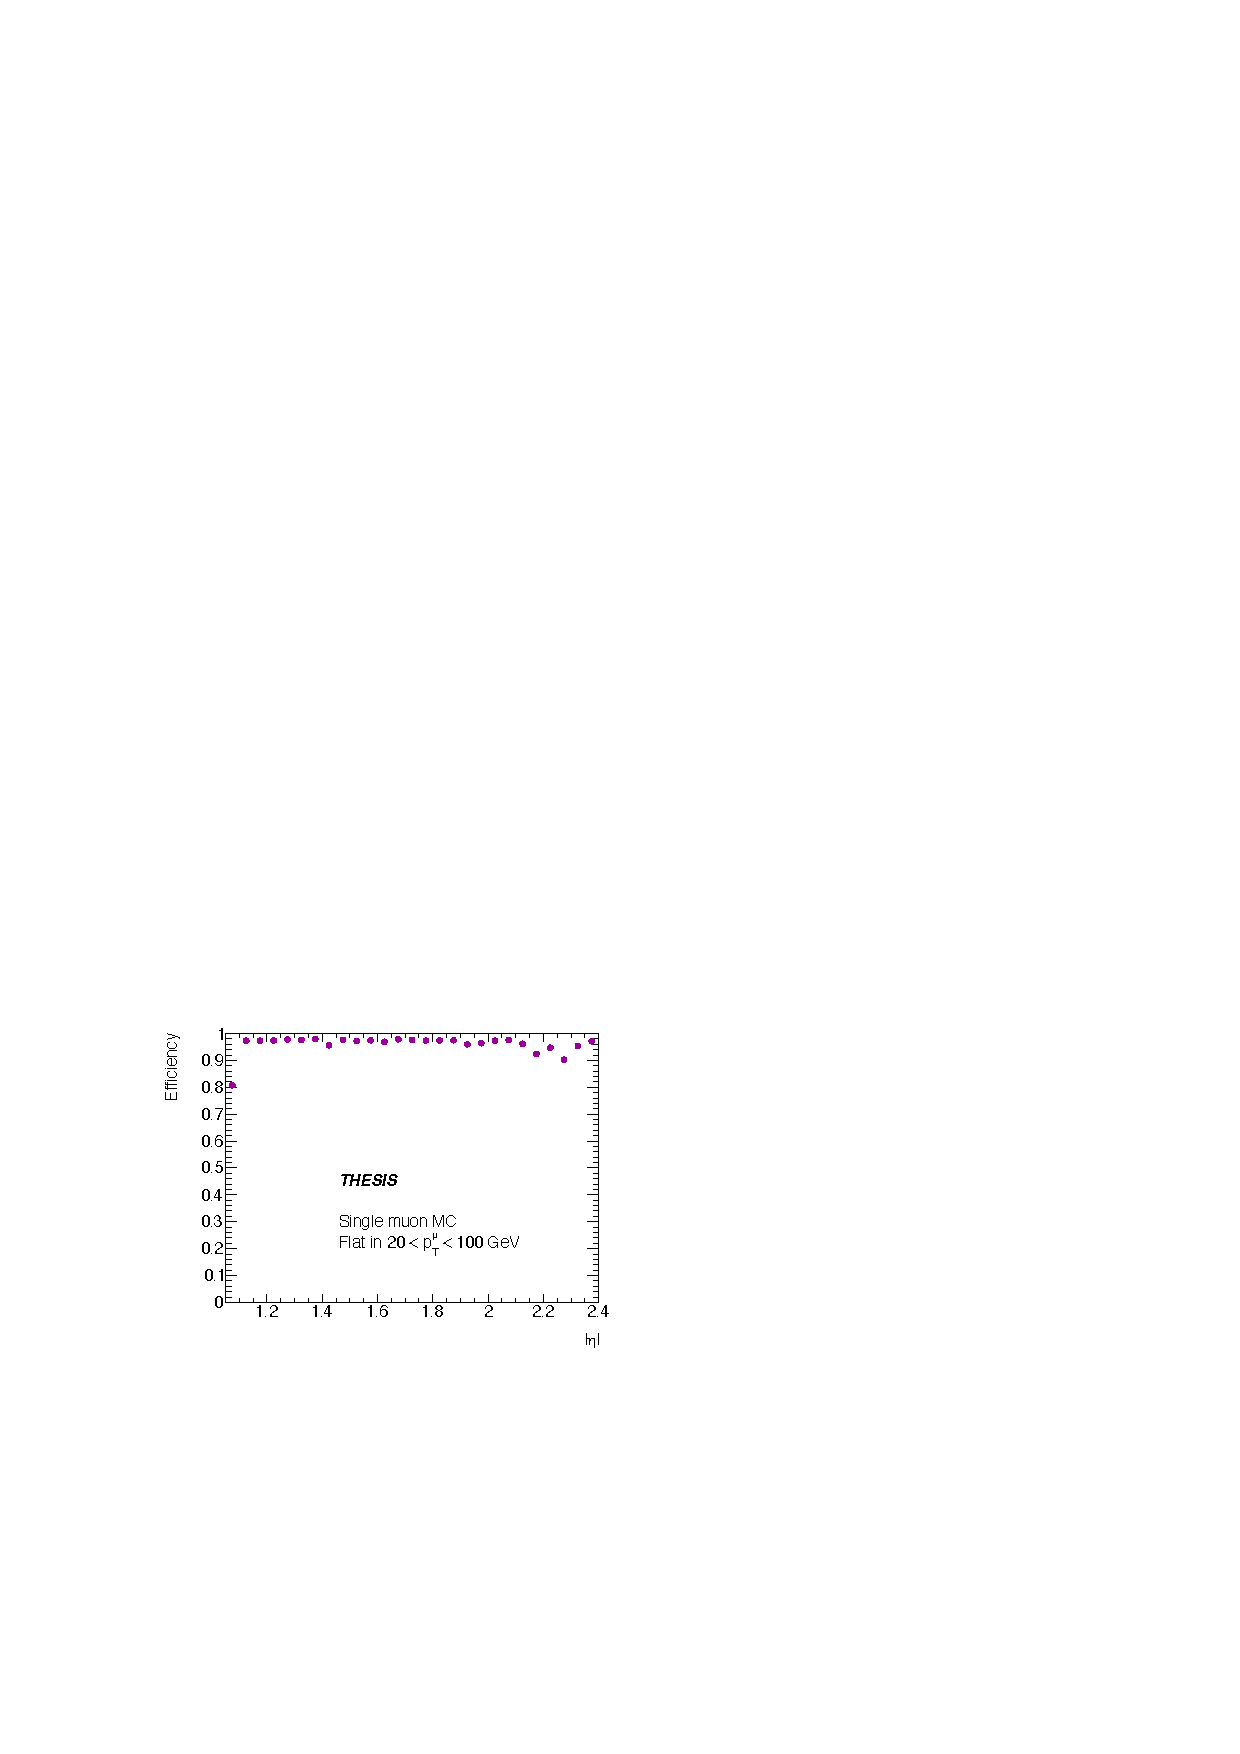
\includegraphics[height=6cm]{fig/Test/Vivado_Wire_eta.pdf}
\subcaption{Efficiencyの$\eta$依存性}
\end{minipage}%
\begin{minipage}[b]{.5\linewidth}
\centering
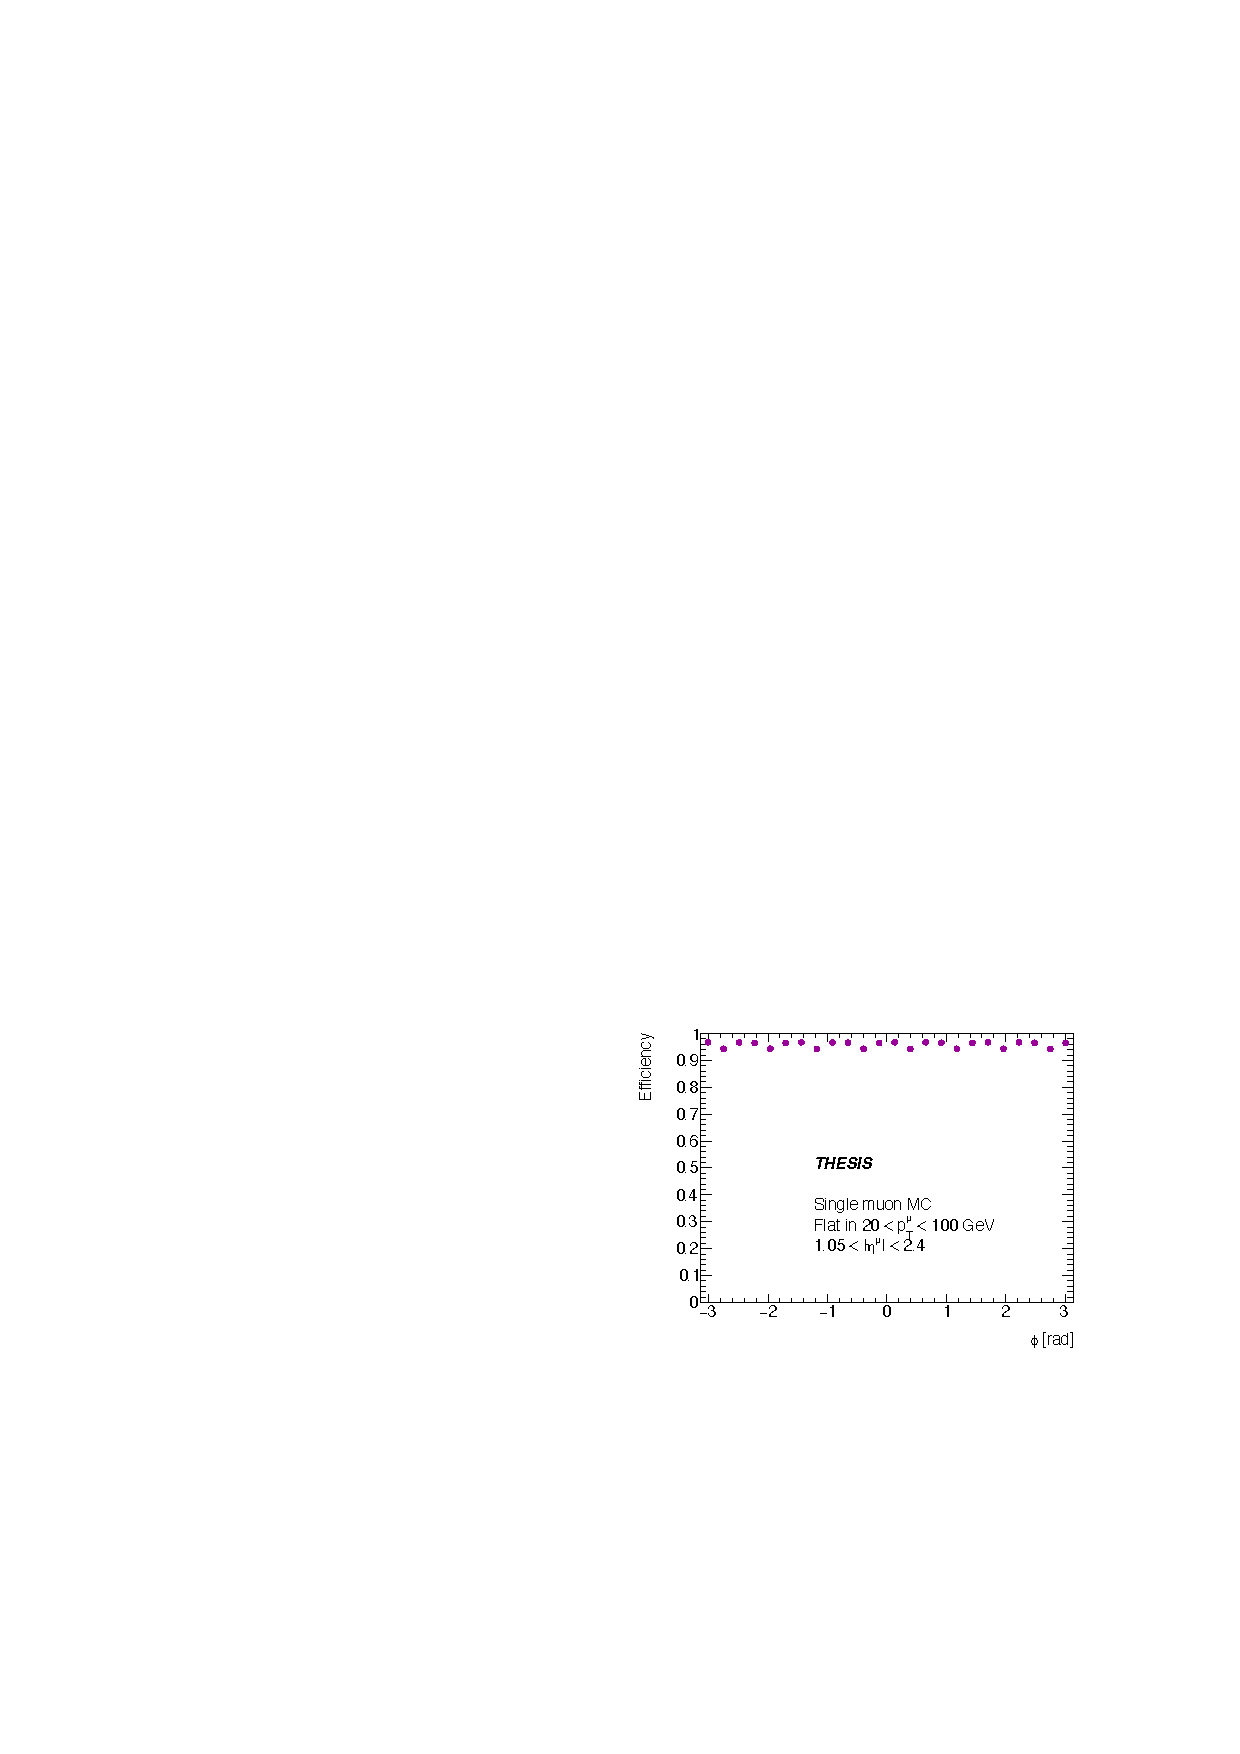
\includegraphics[height=6cm]{fig/Test/Vivado_Wire_phi.pdf}
\subcaption{Efficiencyの$\phi$依存性}
\end{minipage}%
\caption[Wire Segment Reconstructionの検出効率]{Wire Segment Reconstructionの検出効率\cite{mt_nabeyama}}
\label{Vivado_Wire_Efficiency}
\end{figure}

\begin{equation}
\mathrm{Efficiency} = \frac{\mathrm{Wire \,Segment \,Reconstructionで}\,\Delta\theta\,\mathrm{を再構成できたイベント数}}{\mathrm{Truth ミューオン の数}}
\end{equation}


TGCチェンバーの構造やエンドキャップマグネットとの干渉によると考えられる、数\%のInefficiencyが局所的に見られるものの、Efficiencyは$\eta$、$\phi$全領域で95 \%程度に達している。これによりWIre Segment ReconstructionのHDL実装が期待通り達成されていることが検証された。

HDL実装された Strip Segment Reconstruction と Wire strip Coincidence の動作検証は、ソフトウェアシミュレーターの出力との一致を確かめることで行われた。Strip Segment Reconstruction ではソフトウェアシミュレーターによるStrip Station Coincidenceの出力をインプットとして利用し、Segment Reconstruction の出力をソフトウェアシミュレーターとVivado シミュレーターで比較している。比較結果を表\ref{tab:Vivado_strip}に示す。エンドキャップ領域 (EC) 、フォワード領域 (FW)それぞれで出力の96 \%程度は一致している。数\%の不一致は、Segment Reconstructionをパスした飛跡候補が複数あった場合にどれを優先的に後段に送るか、という候補選択ロジックの差異によるものであると理解されている。同じユニット内でヒットレイヤー数が同じ、かつユニット中心からの距離も同じである候補が存在する場合、HDLではM3 スタッガードチャンネルの上位bitを優先に選ぶ、というロジックが実装されているがソフトウェアシミュレーターではその二つを仕分ける方法を用意するのが原理的に困難である。


\begin{table}[]
    \centering
    \caption*{Strip Segment Reconstruction出力のソフトウェアシミュレーターとVivadoシミュレーター比較結果。ECはエンドキャップ領域、FWはフォワード領域を示す。\cite{mt_kawamoto}}
    \label{tab:Vivado_strip}
    \begin{tabular}{|c|cc|}
    \hline
    \multirow{2}{*}{}        & \multicolumn{2}{c|}{割合}                \\ \cline{2-3} 
                             & \multicolumn{1}{c|}{EC}      & FW      \\ \hline\hline
    飛跡情報が一致したイベント            & \multicolumn{1}{c|}{96.8 \%} & 97.8 \% \\ \hline
    候補の選び方の違いに由来する差異があったイベント & \multicolumn{1}{c|}{3.2 \%}  & 2.2 \%  \\ \hline
    候補の選び方以外に由来する差異があったイベント  & \multicolumn{1}{c|}{1.8 \%}  & 0 \%    \\ \hline
    \end{tabular}
\end{table}

Wire Strip Segment Reconstruction はソフトウェアシミュレーターのWire Segment Reconstruction、Strip Segment Reconstruction の出力を取り出してインプットとしている。比較結果を表\ref{tab:Vivado_WS}に示す。同様のわずかなロジックの違いによる出力の不一致は存在するが、おおむねソフトウェアで設計されたロジックと同等のものをHDLで実装できていることが確認された。

% Please add the following required packages to your document preamble:
% \usepackage{multirow}
\begin{table}[]
    \centering
    \caption*{Wire Strip Coincidence出力のソフトウェアシミュレーターとVivadoシミュレーター比較結果。ECはエンドキャップ領域、FWはフォワード領域を示す。\cite{mt_kawamoto}}
    \label{tab:Vivado_WS}
    \begin{tabular}{|c|cc|}
    \hline
    \multirow{2}{*}{}                      & \multicolumn{2}{c|}{割合}                \\ \cline{2-3} 
                                           & \multicolumn{1}{c|}{EC}      & FW      \\ \hline\hline
    飛跡情報が一致したイベント                          & \multicolumn{1}{c|}{98.4 \%} & 99.9 \% \\ \hline
    飛跡情報の異なったイベント                          & \multicolumn{1}{c|}{1.6 \%}  & 0.07 \% \\ \hline
    イベントで最大の\textbackslash{}pt出力がことなったイベント & \multicolumn{1}{c|}{0.09 \%} & 0.02 \% \\ \hline
    \end{tabular}
\end{table}

\subsection*{トリガーロジックのハードウェアでの実現}
最後にRTLで実装されたトリガー論理回路をハードウェア上で実現するためのインプリメンテーション作業が行われた。論理回路をハードウェア上で実現するため前章に述べたような、FPGAのリソースやタイミングの制約を満たす形での最適化が行われた。また、トリガー回路へどのように信号を入力し、演算結果をどのように取り出すかという、周辺システムの設計・実装も行われた。

しかし、実機上で動作するトリガー回路の動作検証、性能評価には工夫が必要となる。トリガー回路の入力はPS boardから受信する光信号で、出力はFelixに送信する光信号である。このままではPS boardやFelix、さらに後段の読み出し回路が完成するまで、ハードウェア上で動いているトリガー回路を検証するすべがない。

そこで本研究では、ハードウェア上で動作するトリガー回路にPS boardからの出力をエミュレートしたテストパターンを投入し、その出力をMPSoCから読み出す、シングルボード試験システムを開発した。この試験システムと、先行研究で開発されたテストパターン生成機構を用いることで、トリガー回路を限りなく本番運用に近い形で試験することができる。Vivado シミュレーター、ソフトウェアシミュレーターでこれまで行われていた試験と、本システムで達成する試験システムのフローの違いを図\ref{Test_Flow}に示す。

\begin{figure}
\begin{minipage}[b]{0.9\linewidth}
\centering
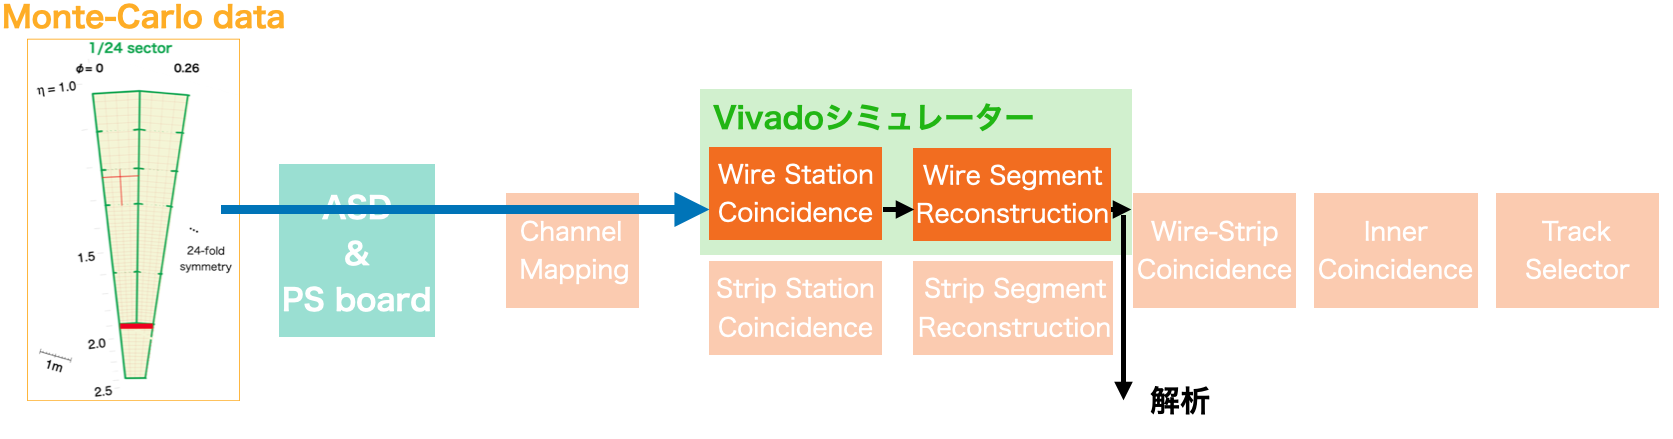
\includegraphics[height=4.8cm]{fig/Test/Flow_Wire.png}
\subcaption{Vivadoシミュレーターによる試験フロー : Wire Segment Reconstruction}
\end{minipage}\\
\begin{minipage}[b]{0.9\linewidth}
    \centering
    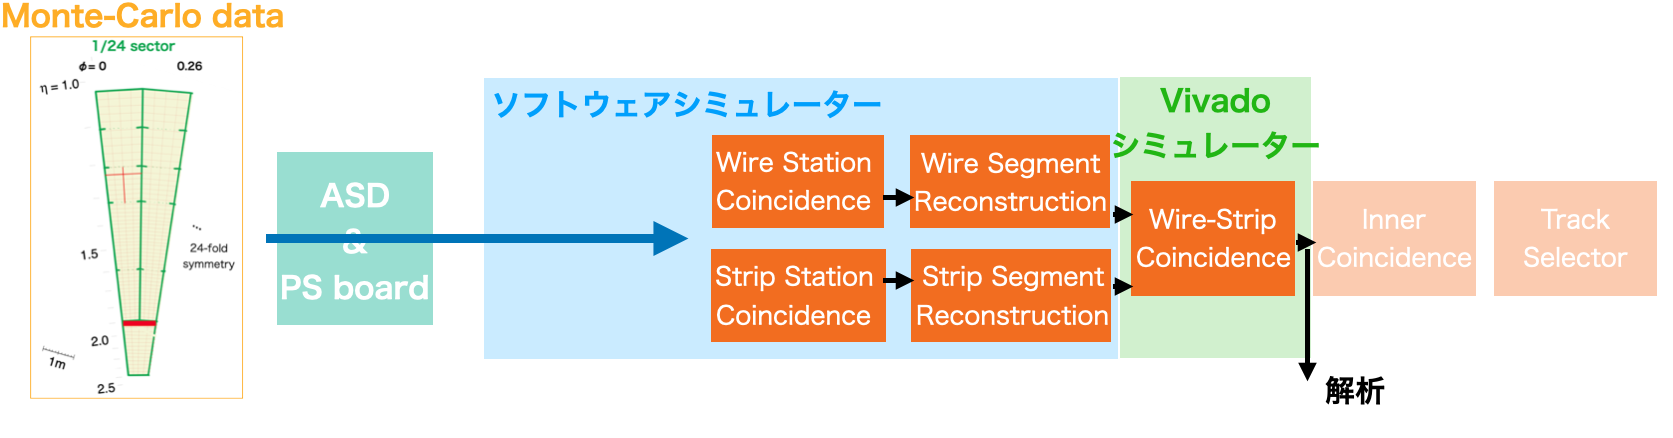
\includegraphics[height=4.8cm]{fig/Test/Flow_WS.png}
    \subcaption{Vivadoシミュレーターによる試験フロー : Wire Strip Coincidence}
\end{minipage}\\
    \begin{minipage}[b]{0.9\linewidth}
        \centering
        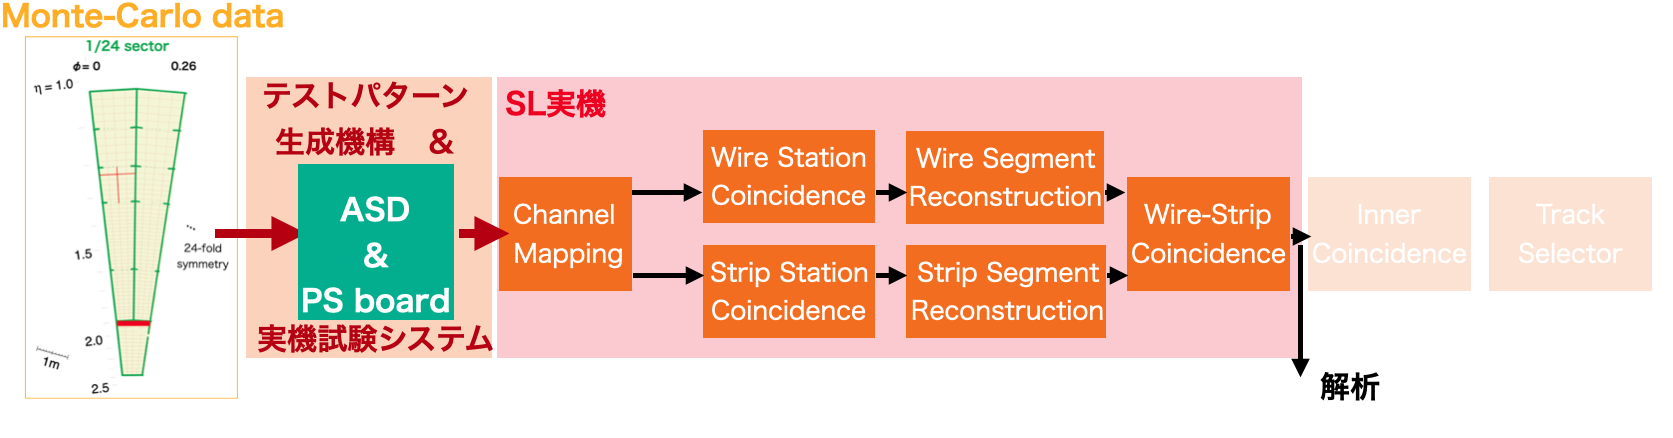
\includegraphics[height=4.8cm]{fig/Test/Flow_zikki.png}
        \subcaption{実機試験システムによる試験フロー}
    \end{minipage}\\

\caption[試験フロー]{Vivado シミュレーター、ソフトウェアシミュレーターによる試験フローと実機試験フローの比較。}
\label{Test_Flow}
\end{figure}


これまでの試験はMCサンプルやソフトウェアシミュレーターから、各モジュールのインプットを直接生成し、トリガーロジックの一部分のHDLをVivadoシミュレーターで試験していた。本試験システムではTGCのヒット情報から、フロントエンドエレクトロニクスの複雑な配線情報も考慮した上で、PS boardからSLに送られる8,000 bitのヒット情報を完全に再現し、トリガーロジックのインプットとする。それをもとにTGC BW コインシデンスをフルチェーンで動作させ、実際にハードウェア上で計算されたトリガー出力を読み出す。また、ソフトウェアシミュレーターではパターンマッチング用のLUTは最終出力のテキストファイルではなく、もととなるrootファイルを利用する。本試験ではいくつかの処理を経て、最終的に出力された本番で使われるテキストファイルを利用するためLUTの最終検査も行うことができる。

さらに、シングルボード試験を実現するには、LUTの書き込みやTTC信号の調整などのコントロールパスと、MPSoCから読み出すための読み出しパスも、トリガー回路と同期しながら精度よく動作する必要があり、SL FPGAの総合的な動作検証を行うことができる。

加えて、実機試験システムはトリガー演算をFPGA上で行っているため、Vivado シミュレーターと比べて高速で動作する。これにより、大統計を活かした網羅的な検証も可能で、これまでVivado シミュレーターでは発見することができなかった局所的な不具合の発見も期待される。\footnote{Vivado シミュレーターはデジタル回路の全ての信号遷移をソフトウェア的に計算するため、回路規模が大きくなると動作が遅くなる。ファームウェア全体をシミュレーションすると、数10イベントに半日程度かかることがわかっており、高統計の試験はできなかった。}

次節で開発した実機試験システムおよびテストパターン生成機構の詳細を説明する。


\section{高輝度LHC-ATLAS実験におけるミューオントリガーロジック}
\label{sec_Phase2TriggerLogic}

前述したように、Phase2 SLは1/24セクター内のTGC BW 7層からのヒット情報を、トリガーをかけることなく受信するようになる。そのためRun3ではトリガー回路はSLB、HPT、SLにまたがって実装されていたが、高輝度LHC-ATLAS実験ではSLのFPGA上に一本化される。高輝度LHC-ATLAS実験におけるミューオントリガー回路の全体像を、図\ref{Trigger_overview}に示す。
トリガー回路はまず、Station CoincidenceおよびSegment reconstructionでワイヤーおよびストリップそれぞれでコインシデンスをとり、$\Delta\theta$および$\Delta\phi$を計算する\footnote{Run3のロジックでは実際の飛跡と無限運動量飛跡を比較する際、M1、M2におけるヒット位置の差分(dR,d$\phi$)を利用していたが、本質的に同じ物理を表している}。次にWire Strip coincidenceにおいて、ワイヤーとストリップ間のコインシデンスをとりミューオンの運動量を概算する。ここでWire Strip coincidenceの出力をTGC track segmentと呼ぶ。TGC track segmentはInner Coincidenceにて、磁場内部の検出器 (NSW、BIS78、RPC、EIL4 TGC、Tile カロリメーター) とコインシデンスを取られ、フェイクトリガーの削減および\pt 精度の向上がなされる。ここまでに最大64個の飛跡候補が提供される。最後にTrack selectorにおいて、64この飛跡候補から\pt の大きさ順に最大6つの飛跡候補が絞られる。そのうち3つはMDTTPに転送する。MDTTPは、この飛跡候補をもとにさらに高い精度でミューオンの運動量を計算し、その結果をSLに送り返す。SLはMDTTPからの飛跡候補と、MDTTPへ転送しなかった飛跡候補のすべてもMUCTPIに転送する。以下に各モジュールの詳細を説明する。


\begin{figure} 
    \centering
    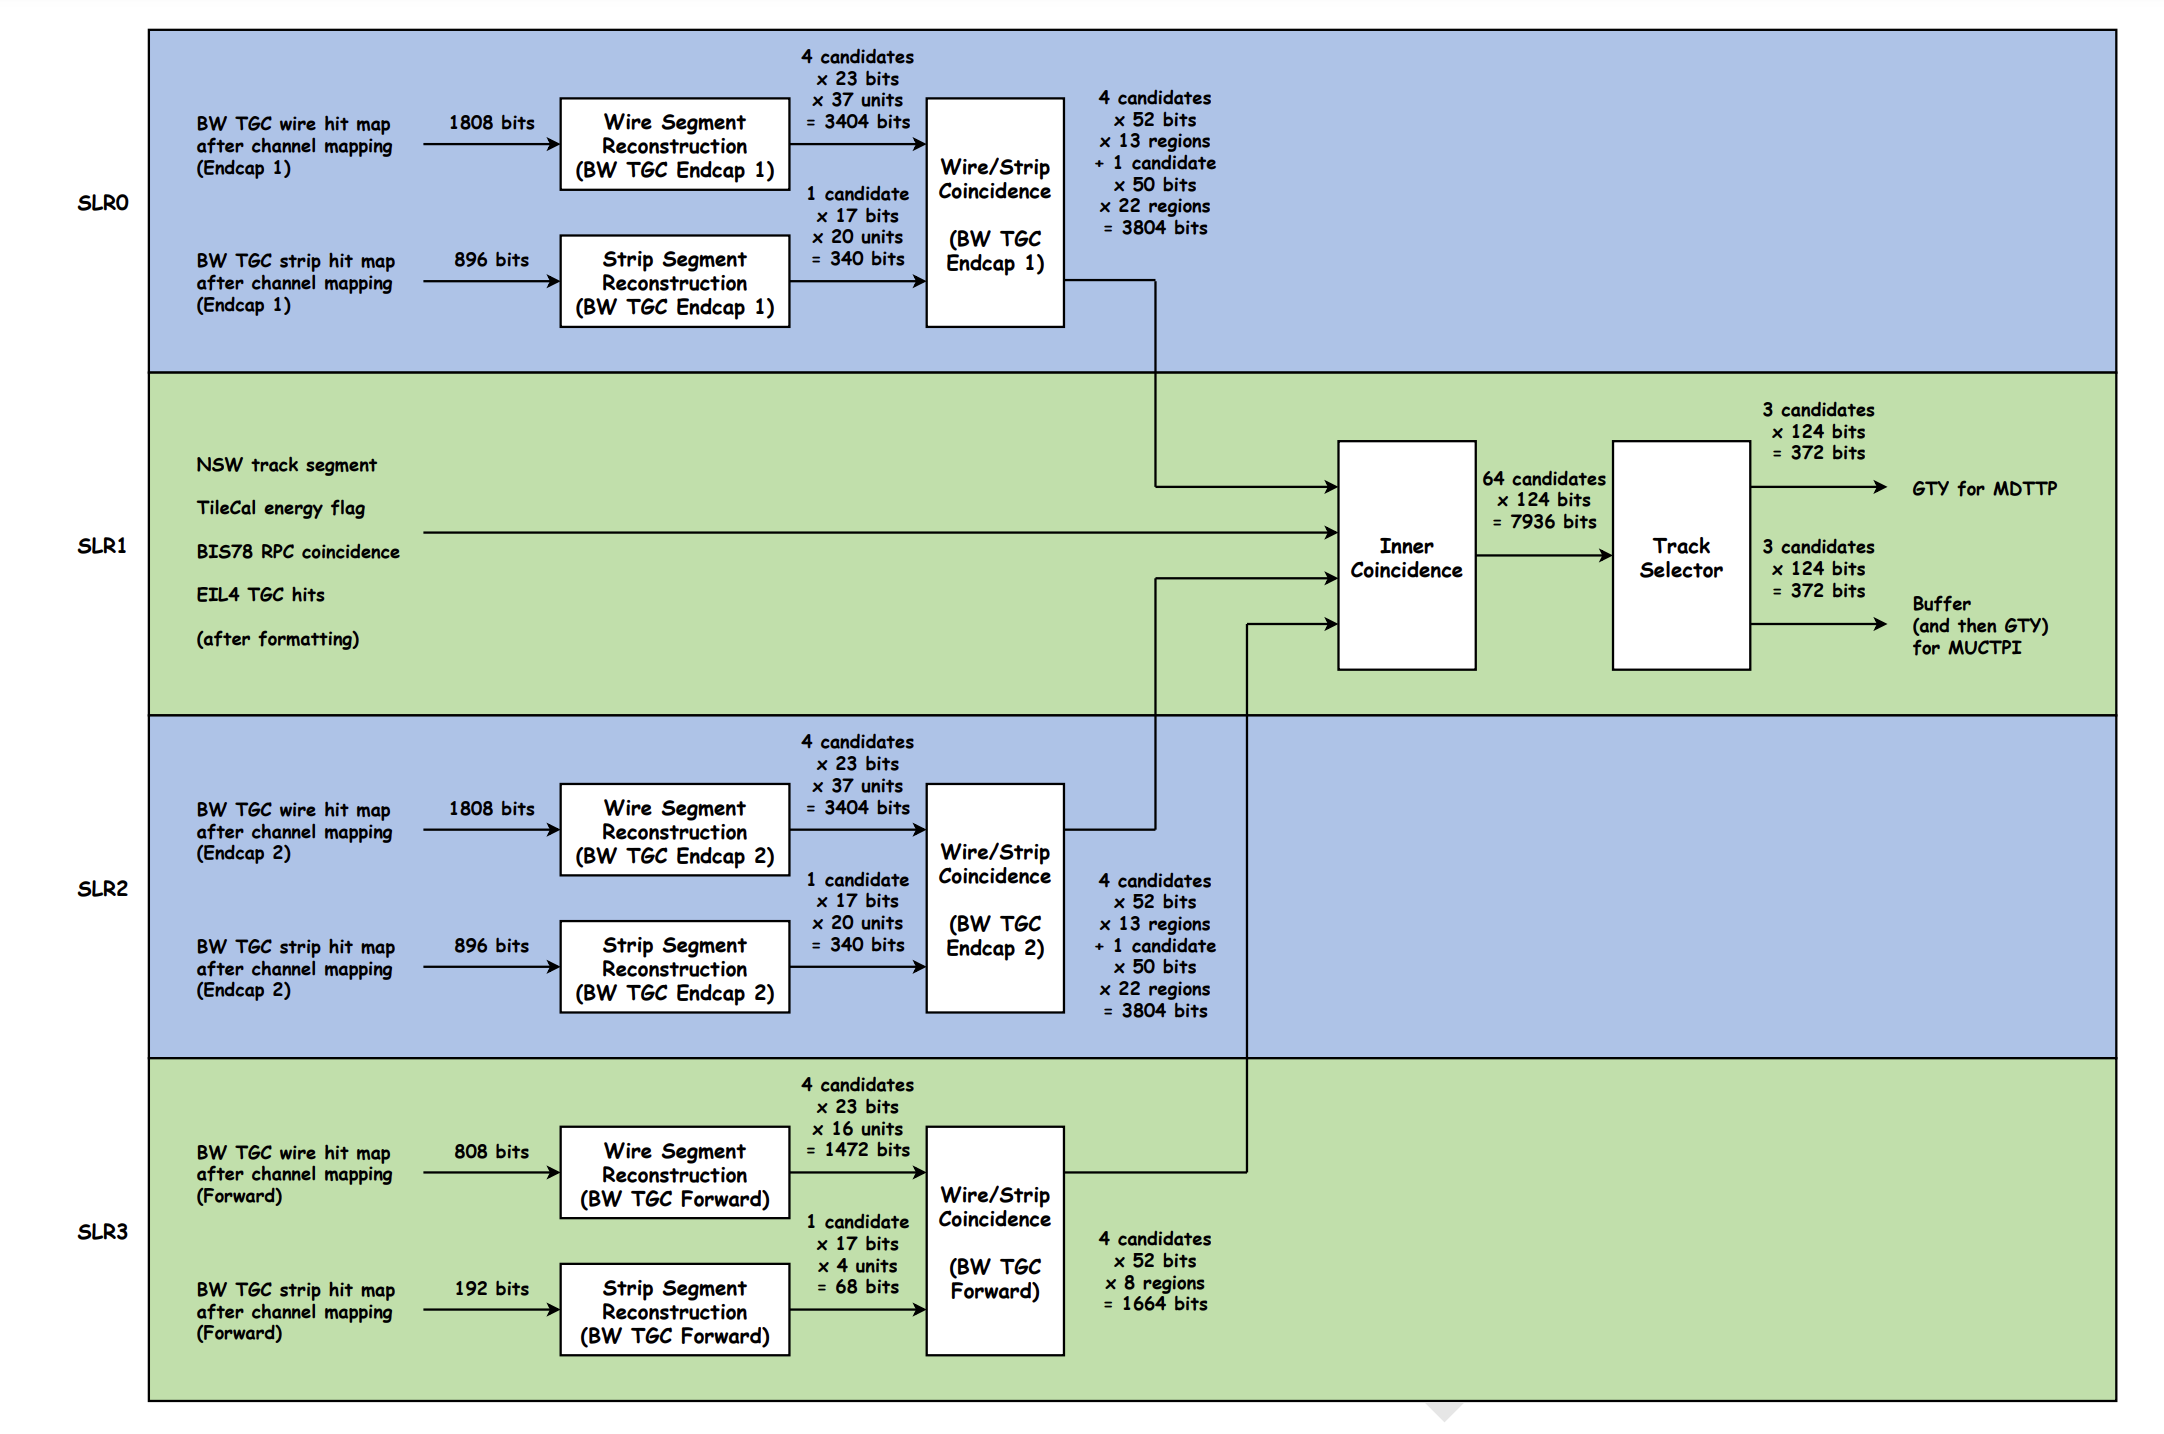
\includegraphics[width=16cm]{fig/SL/Trigger_overview.png}
    \caption[高輝度LHC-ATLAS実験でSLに実装されるトリガーロジックの全体像]{高輝度LHC-ATLAS実験でSLに実装されるトリガーロジック}
    \begin{itembox}{作り直す}
        Station CoincidenceとSegment reconstructionを分けたものに作り直す
    \end{itembox}
    \label{Trigger_overview}
\end{figure}

\begin{itembox}{自分で書き直す}
    一旦、三島さん修論(三島さんはTDRを参考にしている)をそのまま貼っておく。後で自分の言葉で書き直す。コンテンツはこれでOK。
\end{itembox}

\subsection*{Wire Station Coincidence}

このモジュールでは、M1・M2・M3 の各ステーションのそれぞれで、ワイヤーからの信号のコインシデンスをとる。モジュールの駆動クロックは、LHCクロックに同期した周波数 40 MHz のクロックであり、レイテンシは 1 クロックチック分 (25 ns) である。Wire Station Coincidence および Wire Segment Reconstruction におけるロジックでは、Endcap phi0 の領域を 37 ユニット、Endcap phi1 の領域を 37 ユニット、Forward の領域 を 16 ユニットに分割している。ユニットの構造を図\ref{StationCoin_unit}に示す。1 つのユニットは、M1 ステーションでは各層の 32 チャンネルを、M2 ステーションでは各層の 16 チャンネルを、M3 ステーションでは各層の 8 チャンネルをカ バーする。また、1 つのユニットを、そのチャンネル数を 4 等分するようにして 4 つのサブユニットに分割している。各サブユニットの処理は並列して行う。
M1 ステーションにおけるコインシデンスロジックの概要を図 \ref{StationCoin_wire} に示す。全ての層にヒットがある場合 (3/3 コ インシデンス)、2 層のみにヒットがある場合 (2/3 コインシデンス)、1 層のみにヒットがある場合 (1/3 コインシデ ンス) の 3 種類のロジックを用意しており、それぞれを並列に処理する。
M2 および M3 ステーションにおけるコインシデンスロジックの概要を図\ref{StationCoin_doublet}に示す。全ての層にヒットがある 場合 (2/2 コインシデンス)、1 層のみにヒットがある場合 (1/2 コインシデンス) の 2 種類のロジックを用意しており、それぞれを並列に処理する。
M1 および M2 ステーションの各サブユニットの出力は、それが複数の飛跡候補を含んでいる場合は、検出点が ユニットの中心により近いものを 2 つ選択し、Position ID として Wire Segment Reconstruction へ転送する。M3 ステーションの各サブユニットの出力は、それが複数の飛跡候補を含んでいる場合は、$\eta$ がより小さいものを 1 つ 選択し、Position ID として Wire Segment Reconstruction へ転送する。これらのロジックは、より大きな横運動量 をもつミューオンを選択するためのものである。

\begin{figure} 
\centering
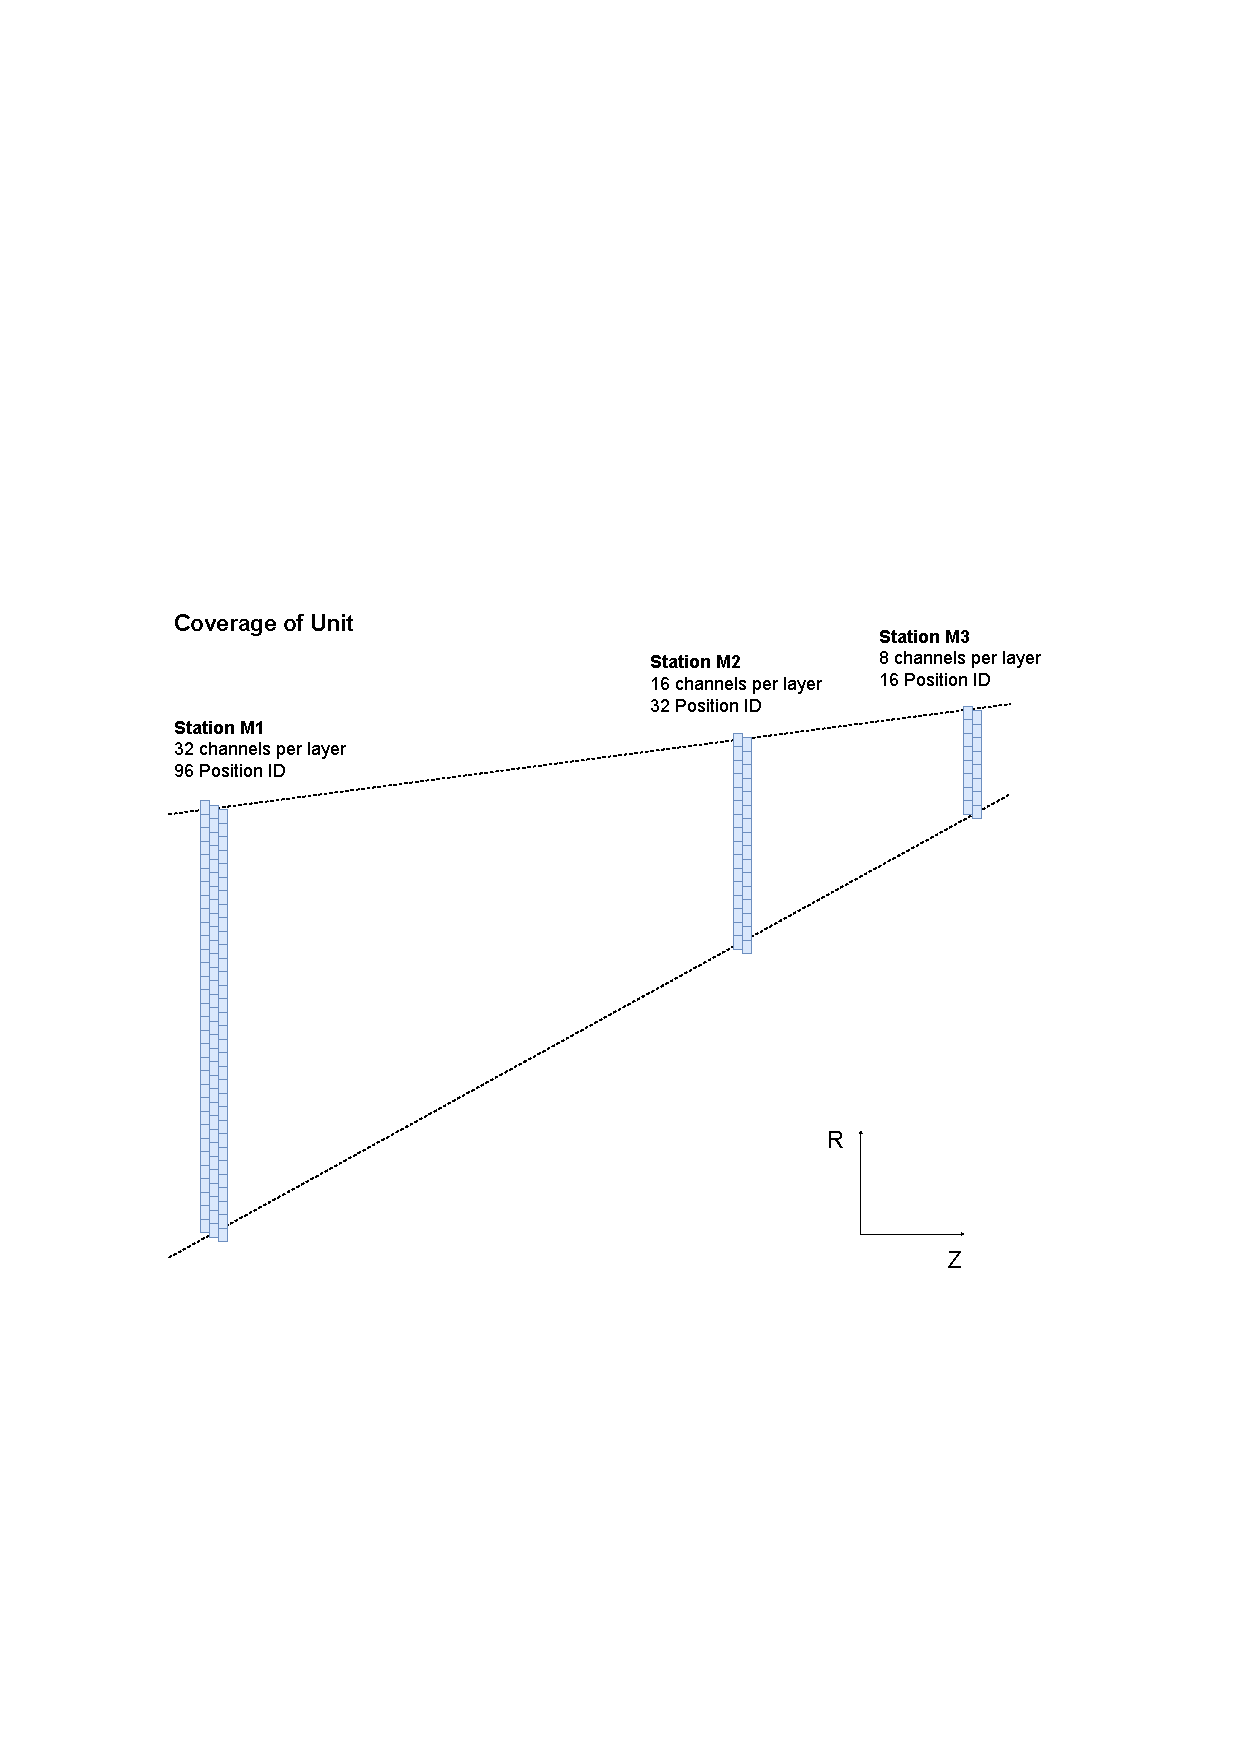
\includegraphics[width=16cm]{fig/SL/StationCoin_unit.pdf}
\caption[Wire Station Coincidence および Wire Segment Reconstruction におけるユニット]{Wire Station Coincidence および Wire Segment Reconstruction におけるユニット}
\label{StationCoin_unit}
\end{figure}

\begin{figure} 
\centering
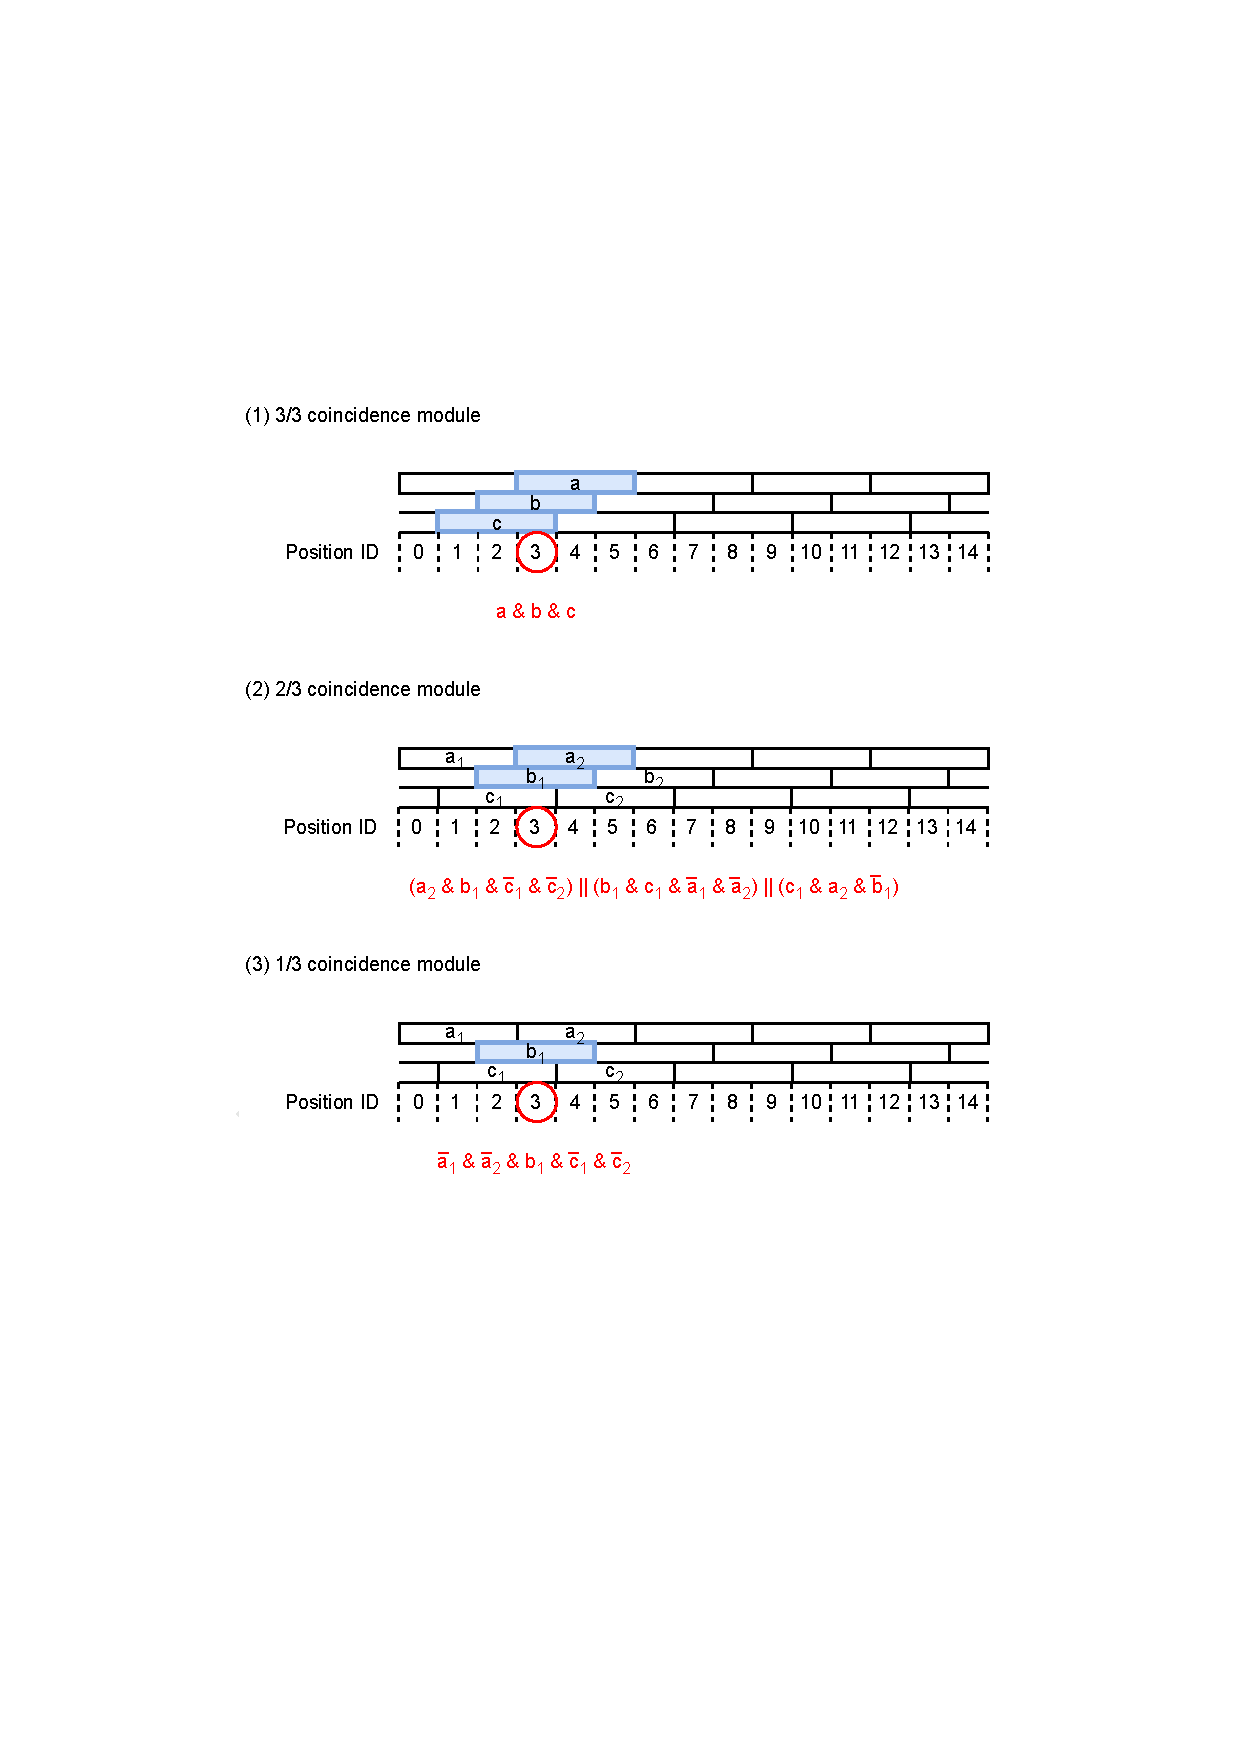
\includegraphics[width=16cm]{fig/SL/StationCoin_wire.pdf}
\caption[M1 tripletにおけるコインシデンスロジック]{M1 tripletにおけるコインシデンスロジック}
\label{StationCoin_wire}
\end{figure}

\begin{figure} 
\centering
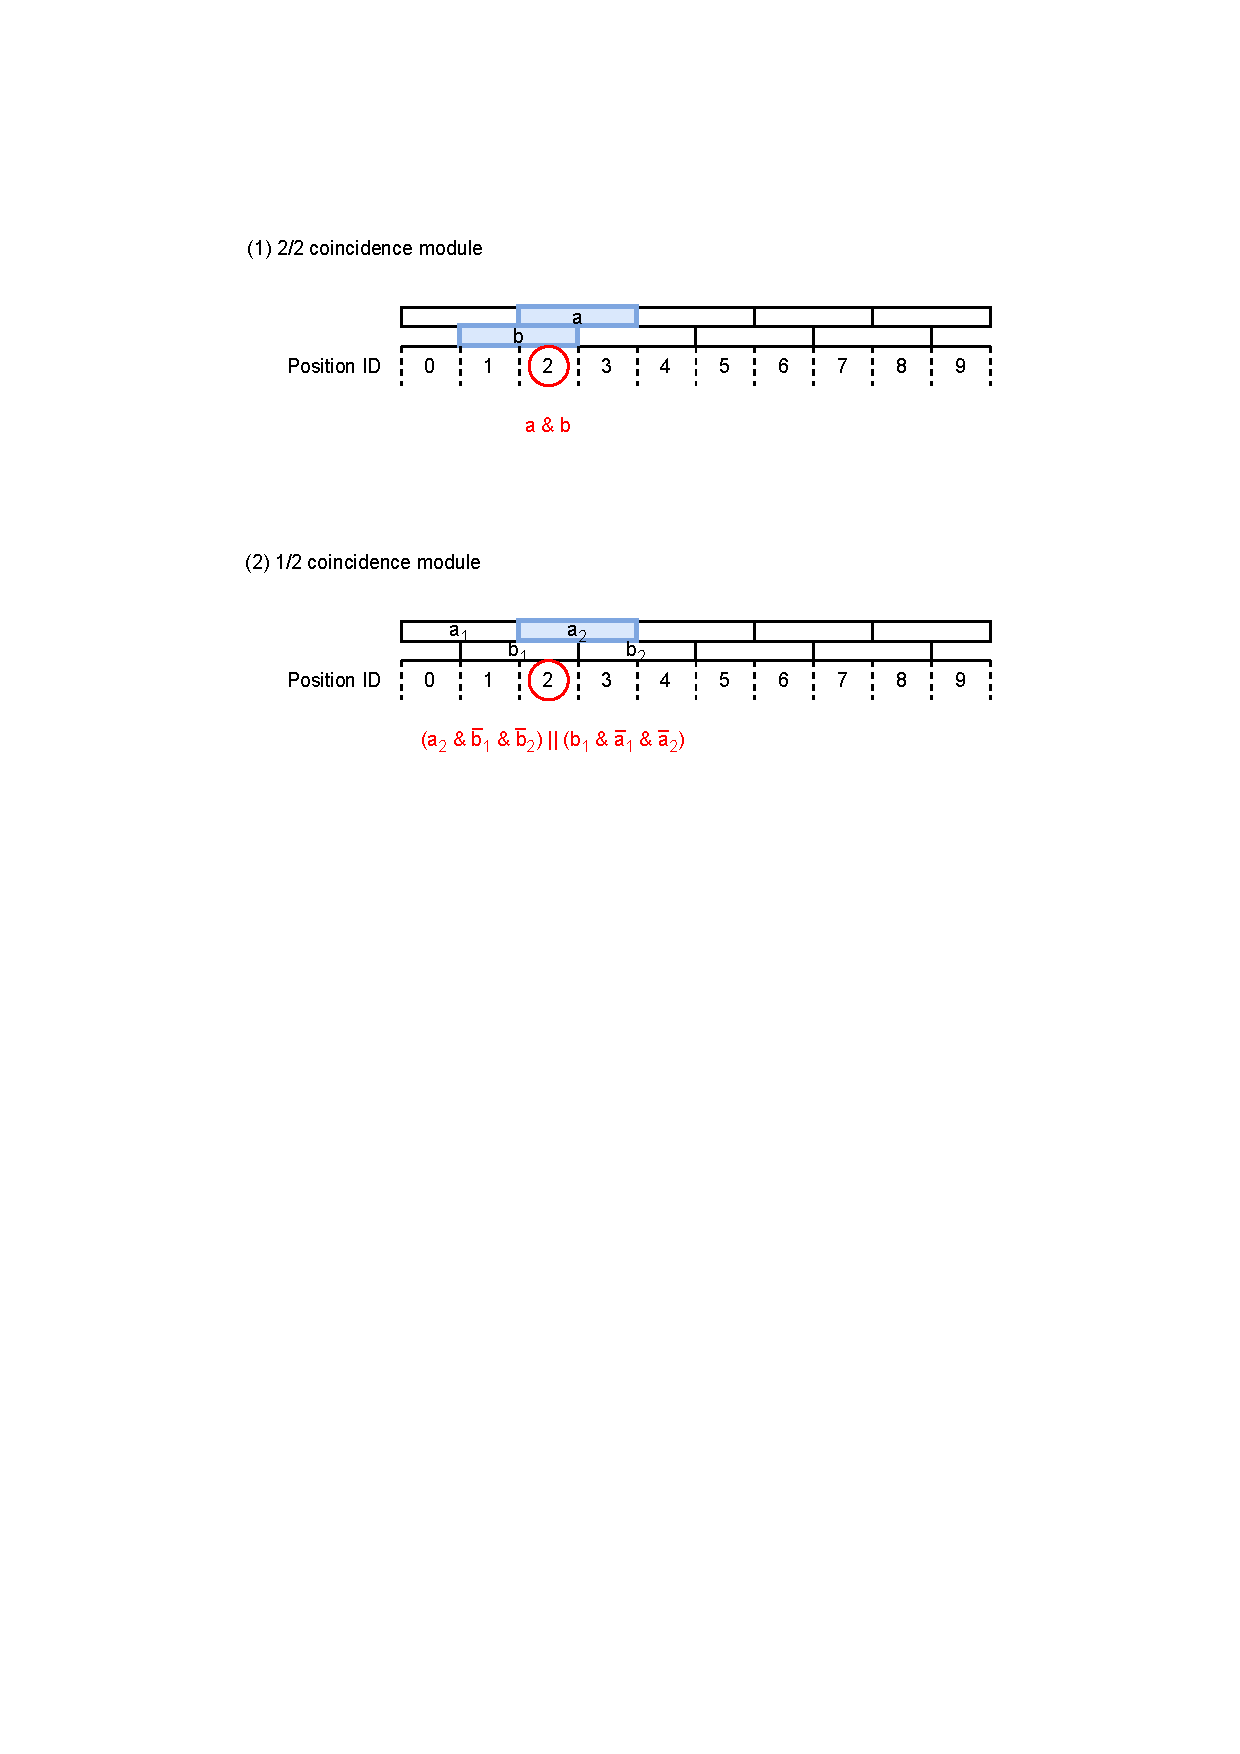
\includegraphics[width=16cm]{fig/SL/StationCoin_doublet.pdf}
\caption[M2・M3 ステーションにおけるコインシデンスロジック]{M2・M3 ステーションにおけるコインシデンスロジック}
\label{StationCoin_doublet}
\end{figure}

\subsection*{Wire Segment Reconstruction}
このモジュールでは、Wire Station Coincidence の結果をもとに、M1・M2・M3 ステーション間のコインシデ ンスをとる。モジュールの駆動クロックは、LHC クロックに同期した周波数 160 MHz のクロックであり、レイテンシーは 12 クロックチック分 (75 ns) である。サブユニット毎のロジックは、Address Specifier・Segment Extractor・Segment Selector から構成している。

\subsubsection*{Address Specifier}
Wire Station Coincidence からの Position ID を、パターンマッチング用の URAM のアドレスに変換し、Segment
Extractor へ送る。コインシデンスロジックの組み合わせによりいくつかのコインシデンスパターンが得られるが、 そのうち表 \ref{tab:StationCoin_wire} に示すパターンのものを、最大で 8 つ転送する。同表において、より上にリストされているコイン シデンスパターンを優先的に選択する。このことは、そのようにすることでより本物に近い位置情報と角度情報を 得られることを示す過去の研究結果に基づく。なお、同表中の Fraction の値は、ミューオンが TGC の各レイヤー にヒットを残す確率がそれぞれ 94\% であると仮定して計算をしたものである。同じコインシデンスパターンが複 数ある場合には、$\eta$がより小さいものを選択する。

\begin{table}[h]
    \centering
    \caption{Wire Station Coincidenceにおけるコインシデンスパターン}
    \label{tab:StationCoin_wire}
    \begin{tabular}{|cc|c|}
    \hline
    \multicolumn{1}{|c|}{\multirow{2}{*}{Coincidence Pattern}} & Hit Pattern & \multirow{2}{*}{Faraction} \\ \cline{2-2}
    \multicolumn{1}{|c|}{}                                     & M1 M2 M3    &                            \\ \hline\hline
    \multicolumn{1}{|c|}{7/7}                                  & 3/3 2/2 2/2 & 0.649                      \\ \hline
    \multicolumn{1}{|c|}{6/7A}                                 & 2/3 2/2 2/2 & 0.124                      \\ \hline
    \multicolumn{1}{|c|}{6/7B}                                 & 3/3 1/2 2/2 & 0.083                      \\ \hline
    \multicolumn{1}{|c|}{6/7C}                        & 3/3 2/2 1/2 & 0.083                      \\ \hline
    \multicolumn{1}{|c|}{5/7A}                                 & 2/3 1/2 2/2 & 0.016                      \\ \hline
    \multicolumn{1}{|c|}{5/7B}                                 & 1/3 2/2 1/2 & 0.016                      \\ \hline
    \multicolumn{1}{|c|}{5/7C}                                 & 3/3 1/2 1/2 & 0.011                      \\ \hline
    \multicolumn{1}{|c|}{5/7D}                                 & 1/3 2/2 2/2 & 0.008                      \\ \hline\hline
    \multicolumn{2}{|c|}{Total}                                              & 0.988                      \\ \hline
    \end{tabular}
    \end{table}

\subsubsection*{Segment Extractor}
LUT が格納された URAM のアドレスポートに、Address Specifier からのアドレスを入力し、対応するデータ
(wire segment) を出力する。wire segment のデータフォーマットは表 \ref{tab:WireSegment}に示す通りである。URAM は 2 つの独立に動作するポートを持っており、Address Specifier からの最大 8 つのアドレスを、1 クロックチックに 2 つずつ 処理する。

\begin{table}[h]
    \centering
    \caption{Wire Segmentのフォーマット}
    \label{tab:WireSegment}
    \begin{tabular}{|c|c|}
    \hline
    \# of bits & Name                                                                       \\ \hline\hline
    1          & Flag of successful reconstruction                                          \\ \hline
    2          & Number of the stations with hits used for coincidence                      \\ \hline
    8          & Angle difference $\Delta\theta$ between the segment and the vector from IP \\ \hline
    12         & Global $\eta$ position of the segment                                      \\ \hline
    \end{tabular}
\end{table}

\subsubsection{Segment Selector}
Segment Extractor から送られてくる最大 8 つの wire segment から、サブユニット毎に最大 1 つを選択して出力
する。コインシデンスに用いられてた層の数が多いものを優先して選択する。同じ層の数の wire segment がある 場合には、$\Delta\theta$ がより小さいものを選択する。

\subsection*{Strip Station Coincidence}
このモジュールでは、M1・M2・M3 の各ステーションのそれぞれで、ストリップのコインシデンスをとる。モジュールの駆動クロックは、LHC クロックに同期した周波数 40 MHz のクロックであり、レイテンシは 1 クロックチック分 (25 ns) である。Strip Station Coincidence および Strip Segment Reconstruction におけるロジックでは、Endcap phi0 の領域を 20 ユニット、Endcap phi1 の領域を 20 ユニット、Forward の領域を 4 ユニットに分割している。なお、このユニット数の違いは、エンドキャップ領域では $\eta$ 方向に 5 つのチェンバーが 並んでいることに対して、フォワード領域では 1 つのチェンバーしかないことに由来している。ユニットの構造を
図\ref{StationCoin_unit_strip}  に示す。1 つのユニットは、M1 ステーションでは各層の 20 チャンネルを、M2 ステーションでは各層の 12 チャンネルを、M3 ステーションでは各層の 8 チャンネルをカバーする。また、1 つのユニットを、そのチャンネ ル数を 2 等分するようにして 2 つのサブユニットに分割する。各サブユニットの処理は並列して行う。

ストリップについては、M1・M2・M3 ステーションの全てが 2 層構造になっている。それぞれのステーション
におけるコインシデンスロジックの概要は図\ref{StationCoin_doublet} に示したものと同様である。

\begin{figure} 
\centering
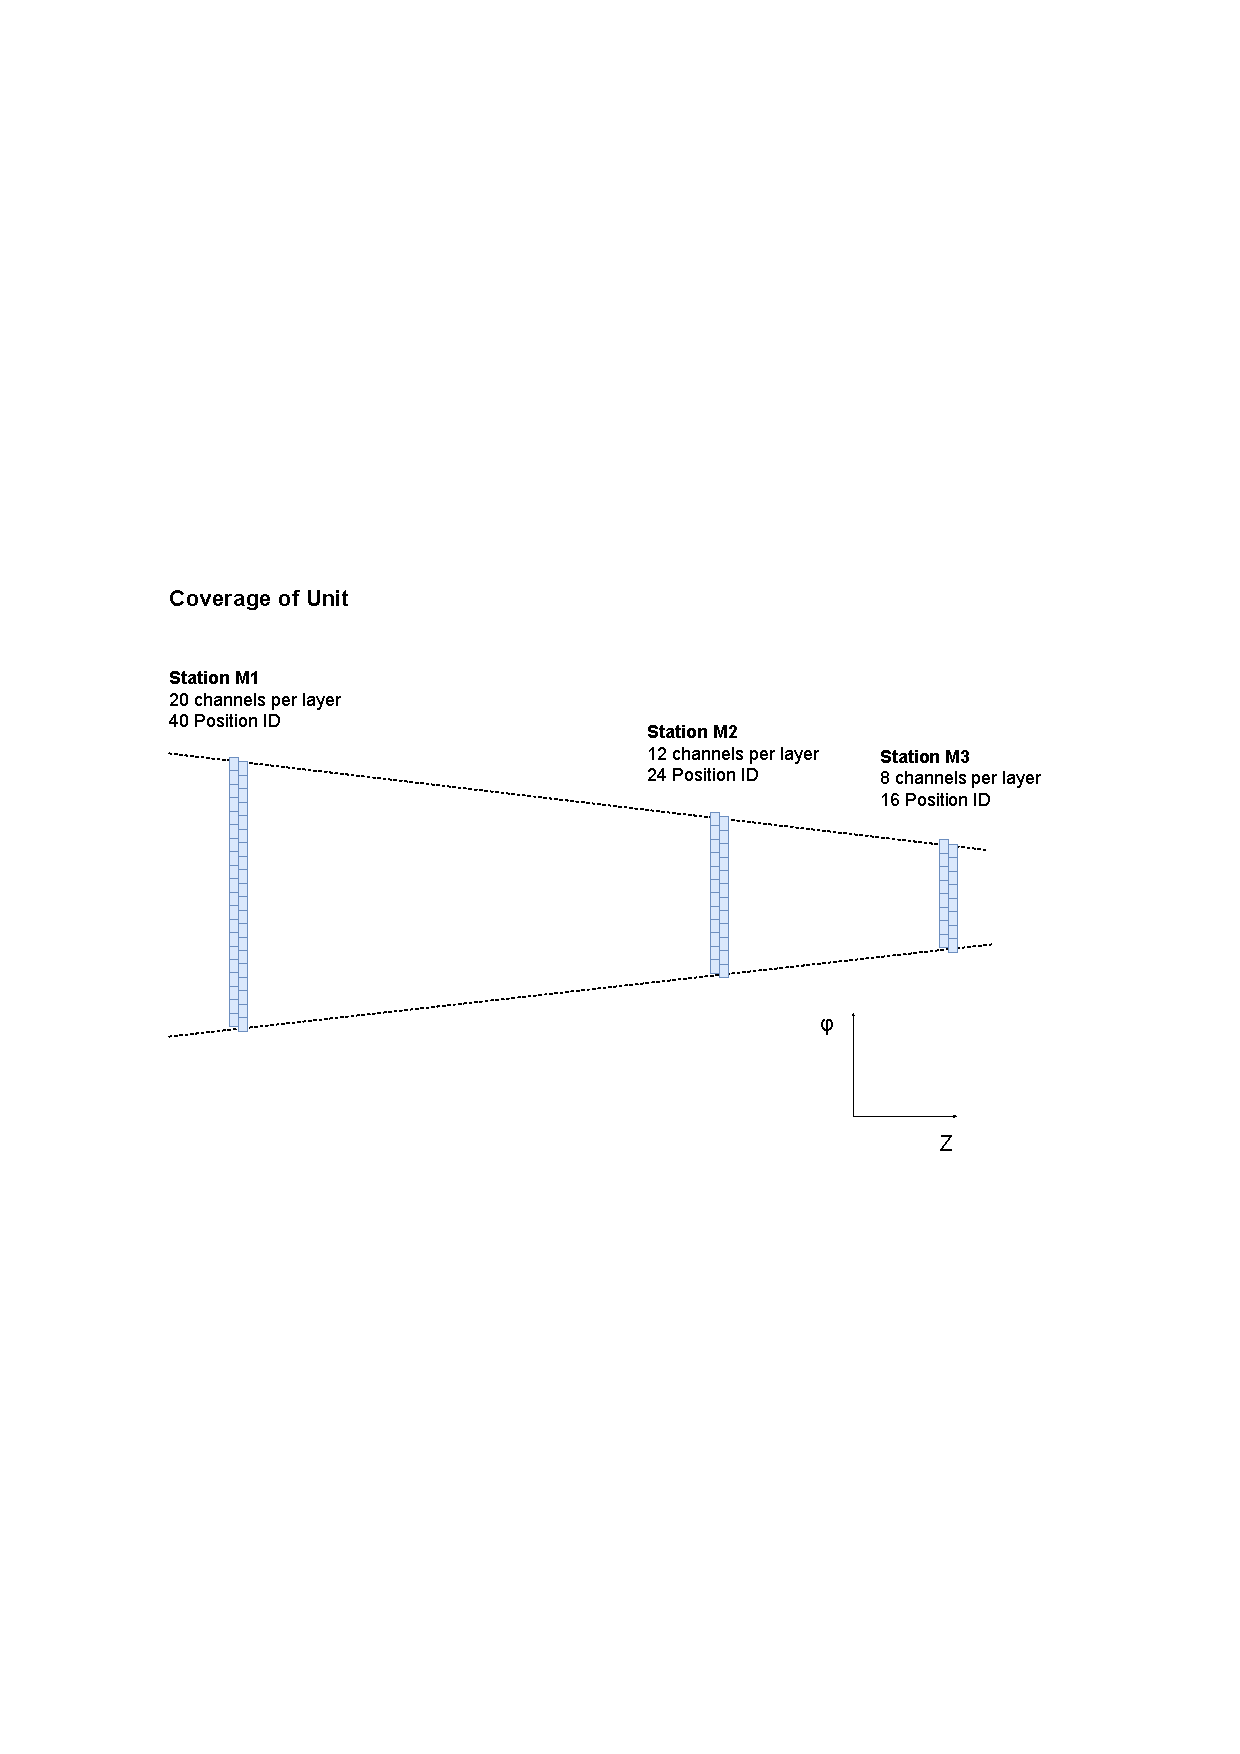
\includegraphics[width=16cm]{fig/SL/StationCoin_unit_strip.pdf}
\caption[Strip Station Coincidence および Strip Segment Reconstruction におけるユニット]{Strip Station Coincidence および Strip Segment Reconstruction におけるユニット}
\label{StationCoin_unit_strip}
\end{figure}

\subsection*{Strip Segment Reconstruction}
このモジュールでは、Strip Station Coincidence の結果をもとに、M1・M2・M3 ステーション間のコインシデンスをとる。モジュールの駆動クロックは、LHC クロックに同期した周波数 240 MHz のクロックであり、レイテ ンシは 21 クロックチック分 (87.5 ns) である。
ユニット毎のロジックを、Address Specifier・Segment Extractor・Segment Selector から構成している。Strip Station Coincidence と合わせたブロックダイアグラムを図 \ref{SegReco_strip} に示す。

\subsubsection*{Address Specifier}
Strip Station Coincidence からの Position ID を、パターンマッチング用の URAM のアドレスに変換し、Segment
Extractor へ送る。コインシデンスロジックの組み合わせによりいくつかのコインシデンスパターンが得られるが、 そのうち表 \ref{tab:SegmentReco_strip} に示すパターンのものを、最大で 6 つ転送する。同表において、より上にリストされているコイン シデンスパターンを優先的に選択する。このことは、そのようにすることでより本物に近い位置情報と角度情報を 得られることを示す過去の研究結果に基づく。

\begin{figure} 
\centering
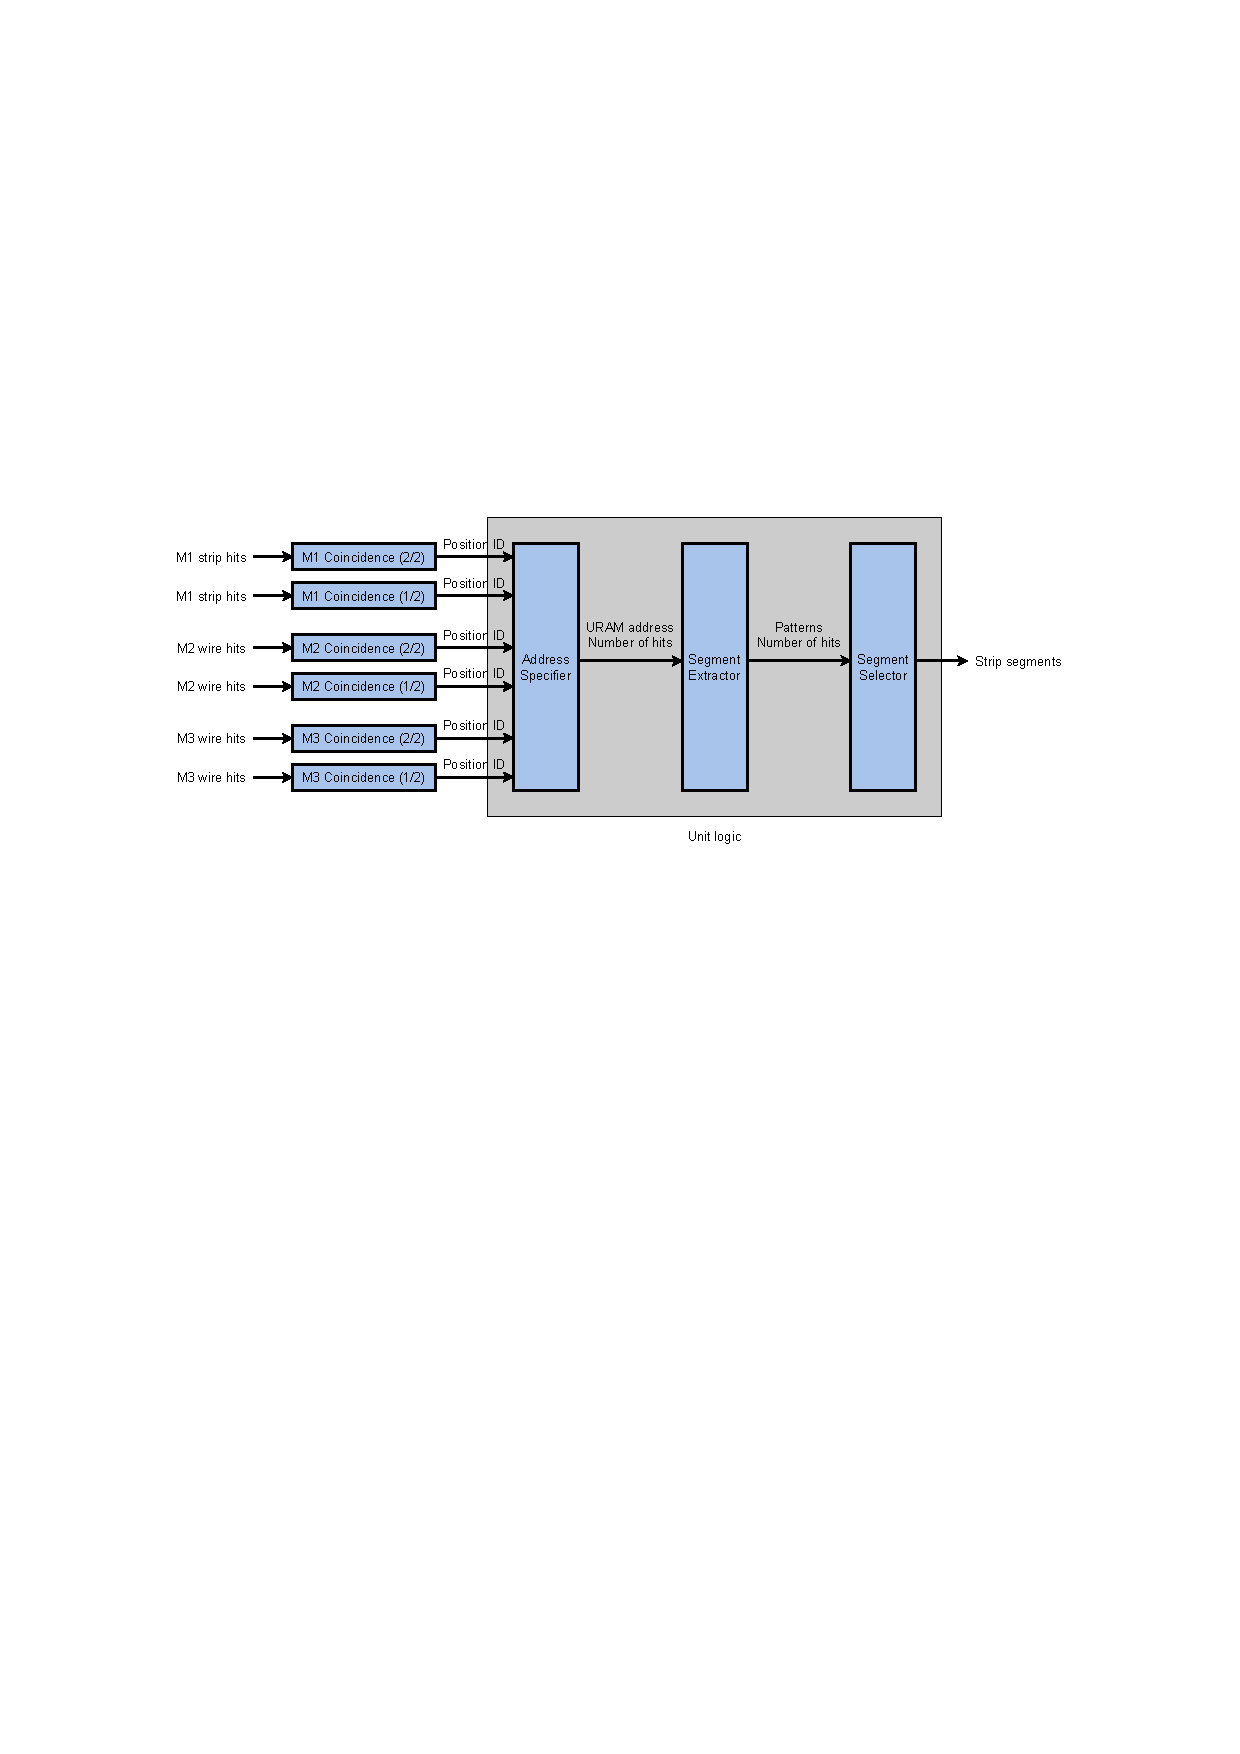
\includegraphics[width=16cm]{fig/SL/SegReco_strip.pdf}
\caption[Strip Segment Reconstruction のブロックダイアグラム]{Strip Segment Reconstruction のブロックダイアグラム}
\label{SegReco_strip}
\end{figure}

\begin{table}[]
    \centering
    \caption{Strip Segment Reconstructionにおけるwire segmentのデータフォーマット}
    \label{tab:SegmentReco_strip}
    \begin{tabular}{|cc|}
    \hline
    \multicolumn{1}{|c|}{\multirow{2}{*}{Coincidence Pattern}} & Hit Pattern \\ \cline{2-2} 
    \multicolumn{1}{|c|}{}                                     & M1 M2 M3    \\ \hline\hline
    \multicolumn{1}{|c|}{6/6}                                  & 2/2 2/2 2/2 \\ \hline
    \multicolumn{1}{|c|}{5/6A}                                 & 2/2 1/2 2/2 \\ \hline
    \multicolumn{1}{|c|}{5/6B}                                 & 1/2 2/2 2/2 \\ \hline
    \multicolumn{1}{|c|}{5/6C}                                 & 2/2 2/2 1/2 \\ \hline
    \multicolumn{1}{|c|}{4/6A}                                 & 1/2 1/2 2/2 \\ \hline
    \multicolumn{1}{|c|}{4/6B}                                 & 2/2 1/2 1/2 \\ \hline
    \multicolumn{1}{|c|}{4/6C}                                 & 1/2 2/2 1/2 \\ \hline\hline
    \multicolumn{2}{|c|}{Total}                                              \\ \hline
    \end{tabular}
\end{table}

\subsubsection*{Segment Extractor}
LUTが格納されたURAMのアドレスポートに、Address Specifierからのアドレスを入力し、対応するデータ (strip segment) を出力する。strip segment のデータフォーマットは表\ref{tab:StripSegment}に示す。URAMは2つの独立に動作するポートを持っており、1 つのポートが1 つのサブユニットを担当している。


\begin{table}[]
    \centering
    \caption{Strip Segmentのフォーマット}
    \label{tab:StripSegment}
    \begin{tabular}{|c|c|}
    \hline
    \# of bits & Name                                                                     \\ \hline\hline
    2          & Number of the stations with hits used for coincidence                    \\ \hline
    6          & Local $\phi$ position in the chamber                                     \\ \hline
    9          & Angle difference $\Delta\phi$ between the segment and the vector from IP \\ \hline
    \end{tabular}
\end{table}

\subsubsection*{Segment Selector}
Segment Extractor から送られてくる最大 6 つの strip segment から、ユニット毎に最大 1 つを選択して出力する。コインシデンスに用いられてた層の数が多いものを優先して選択する。同じ層の数の strip segment がある場
合には、$\Delta\phi$ がより小さいものを選択する。

\subsection*{Wire-Strip Coincidence}
このモジュールでは、wire segment および strip segment 間のコインシデンスをとり、その結果を Inner Coincidence へ転送する。モジュールの駆動クロックは、LHC クロックに同期した周波数 160 MHz のクロックで あり、レイテンシは 6 クロックチック分 (37.5 ns) である。このロジックは、Endcap phi0 を 35 個、Endcap phi1 を 35 個、Forward を 8 個の region に分割し、それぞれを並列に処理する。コインシデンスには、図 \ref{WireStrip_LUT} に示すコインシデンスウィンドウを用いる。
$\Delta\theta$ については、-0.16 <$\Delta\theta$ < 0.16 の領域を 64 ビンに分割している。$\Delta\phi$ に ついては、-0.032 < $\Delta\phi$ < 0.032 の領域を 16 ビンに分割している。
コインシデンスウィンドウの情報は LUT として BRAM に格納する。

\begin{figure} 
\centering
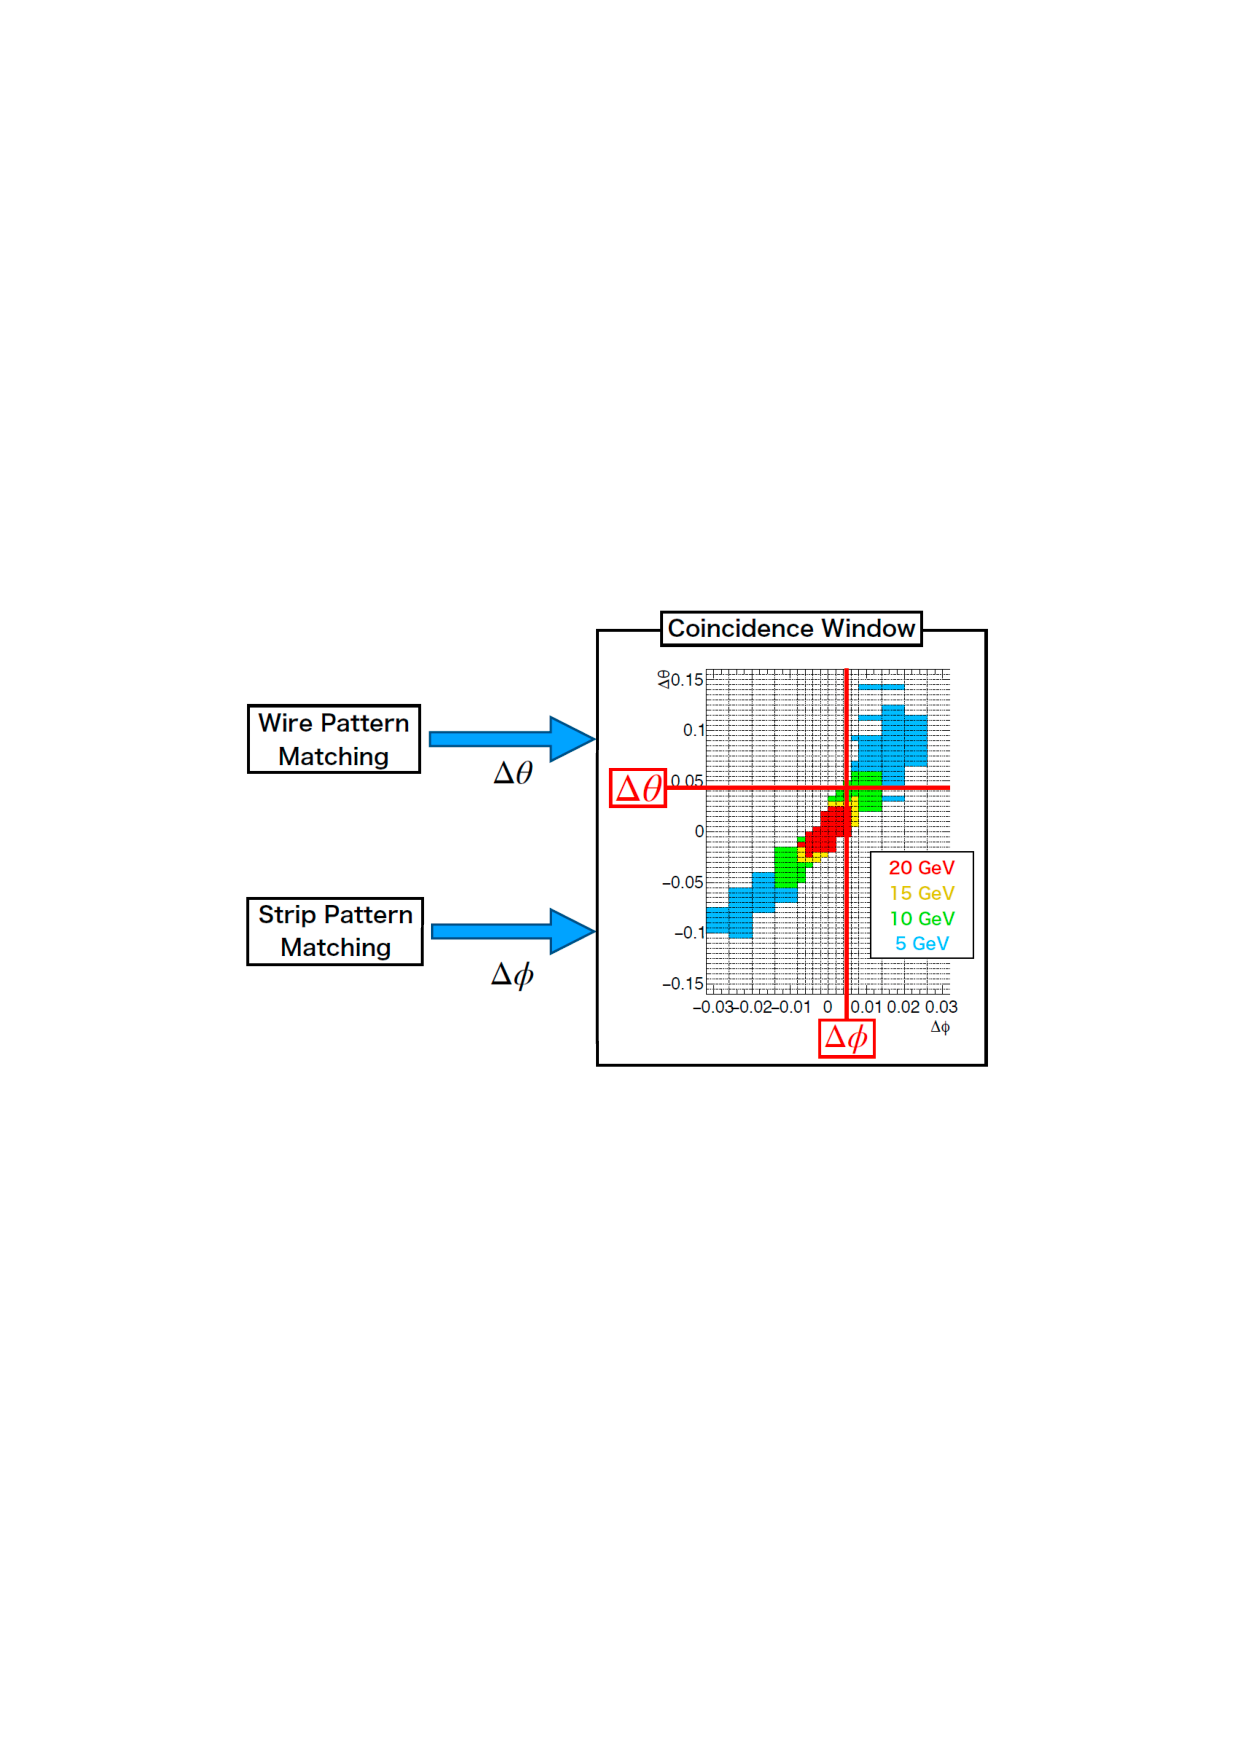
\includegraphics[width=16cm]{fig/SL/WireStrip_LUT.pdf}
\caption[Wire-Strip Coincidence におけるコインシデンスウィンドウ]{Wire-Strip Coincidence におけるコインシデンスウィンドウ}
\label{WireStrip_LUT}
\end{figure}

\subsection*{Inner Coincidence}
このモジュールでは、Wire-Strip Coincidence の出力および内部飛跡検出器 (TGC EIL4・NSW・RPC BIS78・ Tile Calo) からのヒット情報の間のコインシデンスをとり、その結果を Track Selector へ転送する。コインシデンスに用いる LUT は BRAM や URAM に格納する。モジュールの駆動クロックは、LHC クロックに同期した周波 数 320 MHz のクロックであり、レイテンシは 7 クロックチック分 (21.875 ns) である。
図 6.10 に示すように、検出点の $\eta$ および $\phi$、および横運動量 \pt と電荷の正負の情報をもとに、どの内部飛跡検出器の情報をもちいるか選択する。
このロジックは |$\eta$| > 1.3 の領域を 34 個、1.05 < |$\eta$| < 1.3 の領域を 44 個の region に分割し、それぞれを並列 に処理する。最大 64 個の飛跡候補を出力する。飛跡候補のデータフォーマットを表 \ref{tab:InnerCoin} に示す。

\begin{table}[]
    \centering
    \caption{Inner Coincidenceにおける飛跡候補のデータフォーマット}
    \label{tab:InnerCoin}
    \begin{tabular}{|c|c|c|}
    \hline
    \# of bits & Name                             & Comment                                                                \\ \hline\hline
    14         & TGC $\eta$                       & $\eta$ in global candidate at the pivot plane of TGC                   \\ \hline
    9          & TGC $\phi$                       & $\phi$ in global candidate at the pivot plane of TGC                   \\ \hline
    8          & TGC \textbackslash{}pt           & TGC transverse momentum                                                \\ \hline
    4          & TGC \textbackslash{}pt threshold & TGChighest \textbackslash{}pt thresholdsatisfied                       \\ \hline
    1          & TGC charge                       & TGC TC charge                                                          \\ \hline
    3          & Coincidence type                 & Identifier of coincidence type                                         \\ \hline
    14         & MDT $\eta$                       & $\eta$ coordinate of the MDT segment position of the innermost station \\ \hline
    8          & MDT \textbackslash{}pt           & MDT transverse momentum                                                \\ \hline
    4          & MDT \textbackslash{}pt threshold & MDThighesttransversemomentumthresholdsatisfied                         \\ \hline
    1          & MDT charge                       & MDT charge                                                             \\ \hline
    4          & MDT Processing Flag              & Type of reconstructed muon                                             \\ \hline
    2          & \# of segments                   & Number of MDT segments associated to the muon                          \\ \hline
    3          & Segment quality flag             & Quality of each segment                                                \\ \hline
    49         & Reserved                         &                                                                        \\ \hline
    \end{tabular}
\end{table}

\subsection*{Track Selector}
このモジュールでは、InnerCoincidenceから転送される最大64個の飛跡候補から、高いpT をもつものを最大 6 個選択して出力する。モジュールの駆動クロックは、LHC クロックに同期した周波数 160 MHz のクロックであり、レイテンシは 4 クロックチック分 (25 ns) である。
図 \ref{TrackSelector_overview}に示すように、飛跡候補の ID および \pt を選別用の回路に入力する。また、全ての飛跡候補のデータを 選別が完了するまでバッファーする。

\begin{figure} 
    \centering
    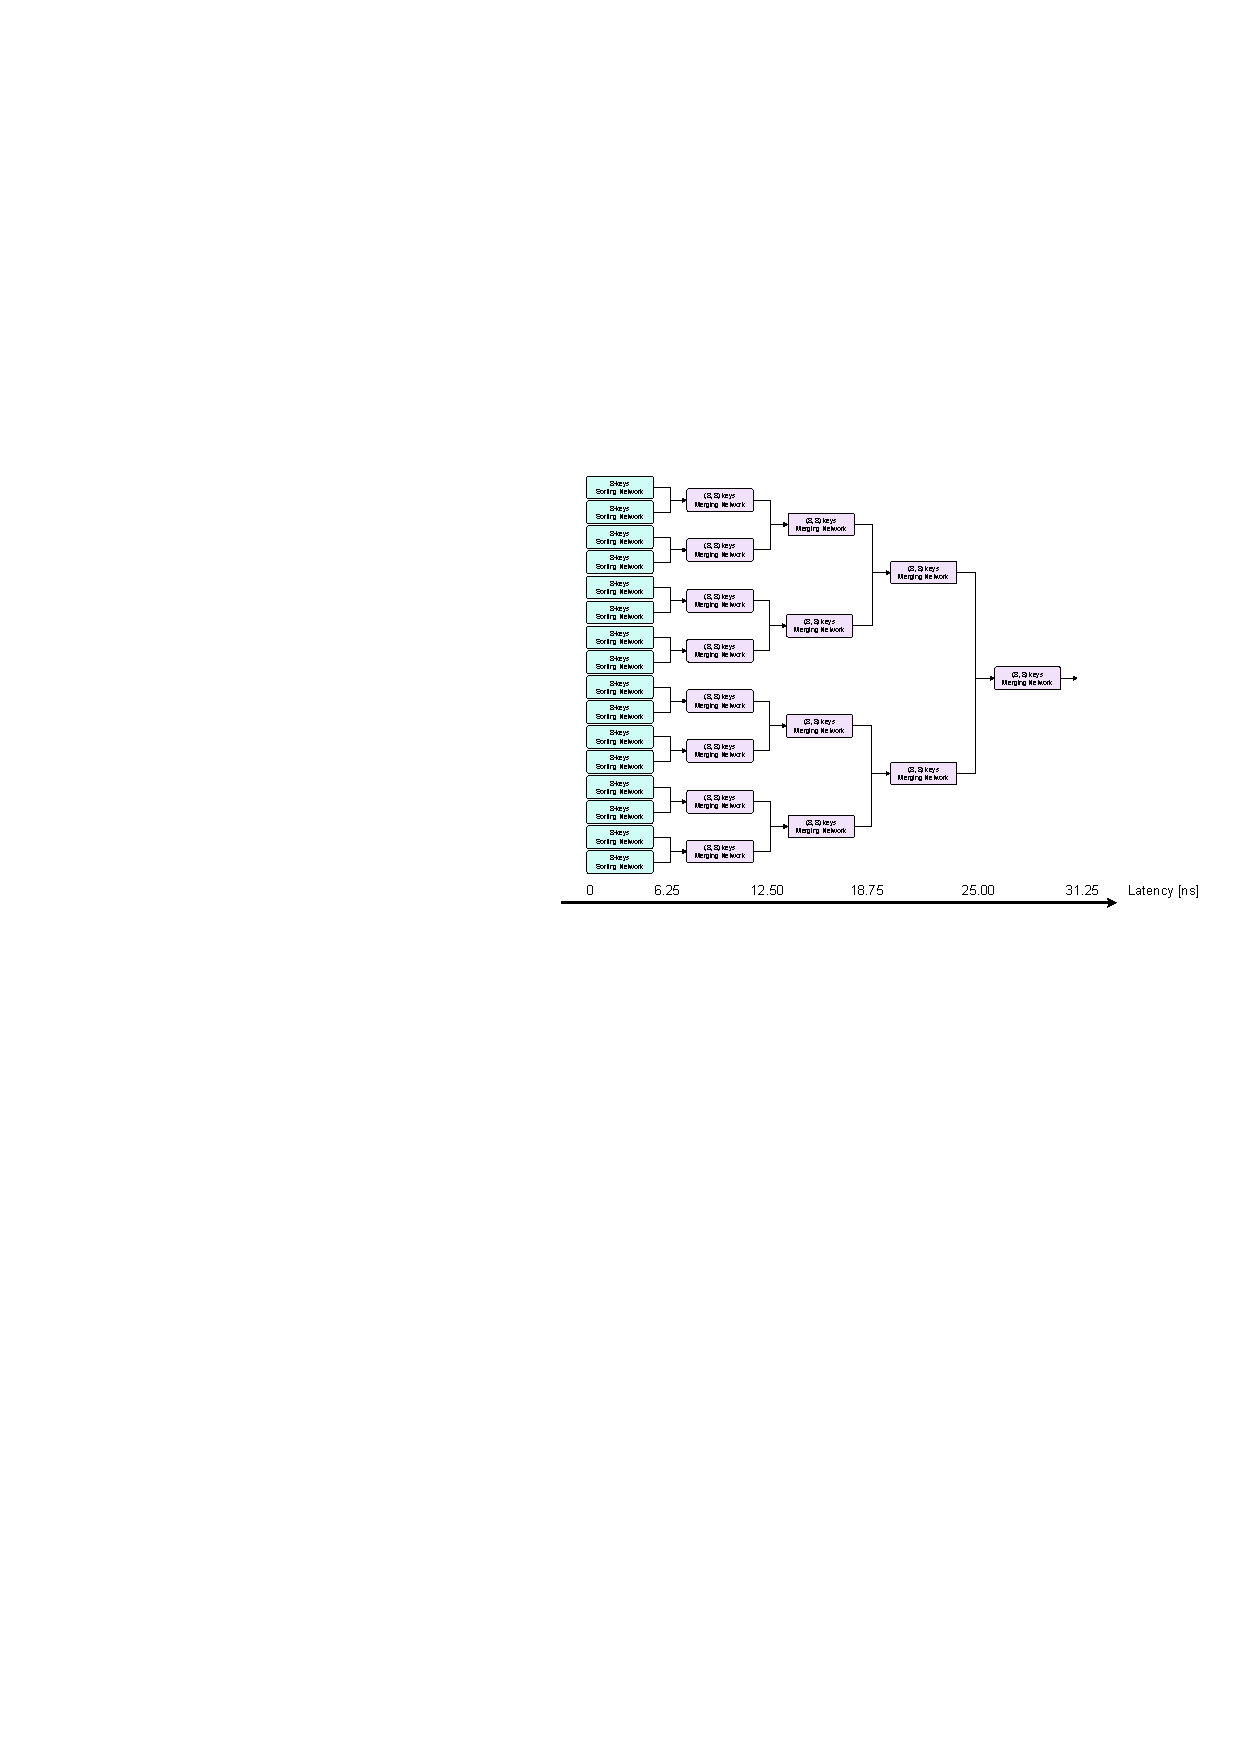
\includegraphics[width=16cm]{fig/SL/TrackSelector_overview.pdf}
    \caption[Track Selector の概要]{Track Selector の概要}
    \label{TrackSelector_overview}
    \end{figure}
    

選別用回路は、図 \ref{TrackSelector} に示すように、8 個の 8-key sorting network および 7 個の 16-key merging network から構成している。全体のレイテンシは 25 ns であり、飛跡候補を 64 個から 8 個まで選別する。

\begin{figure} 
    \centering
    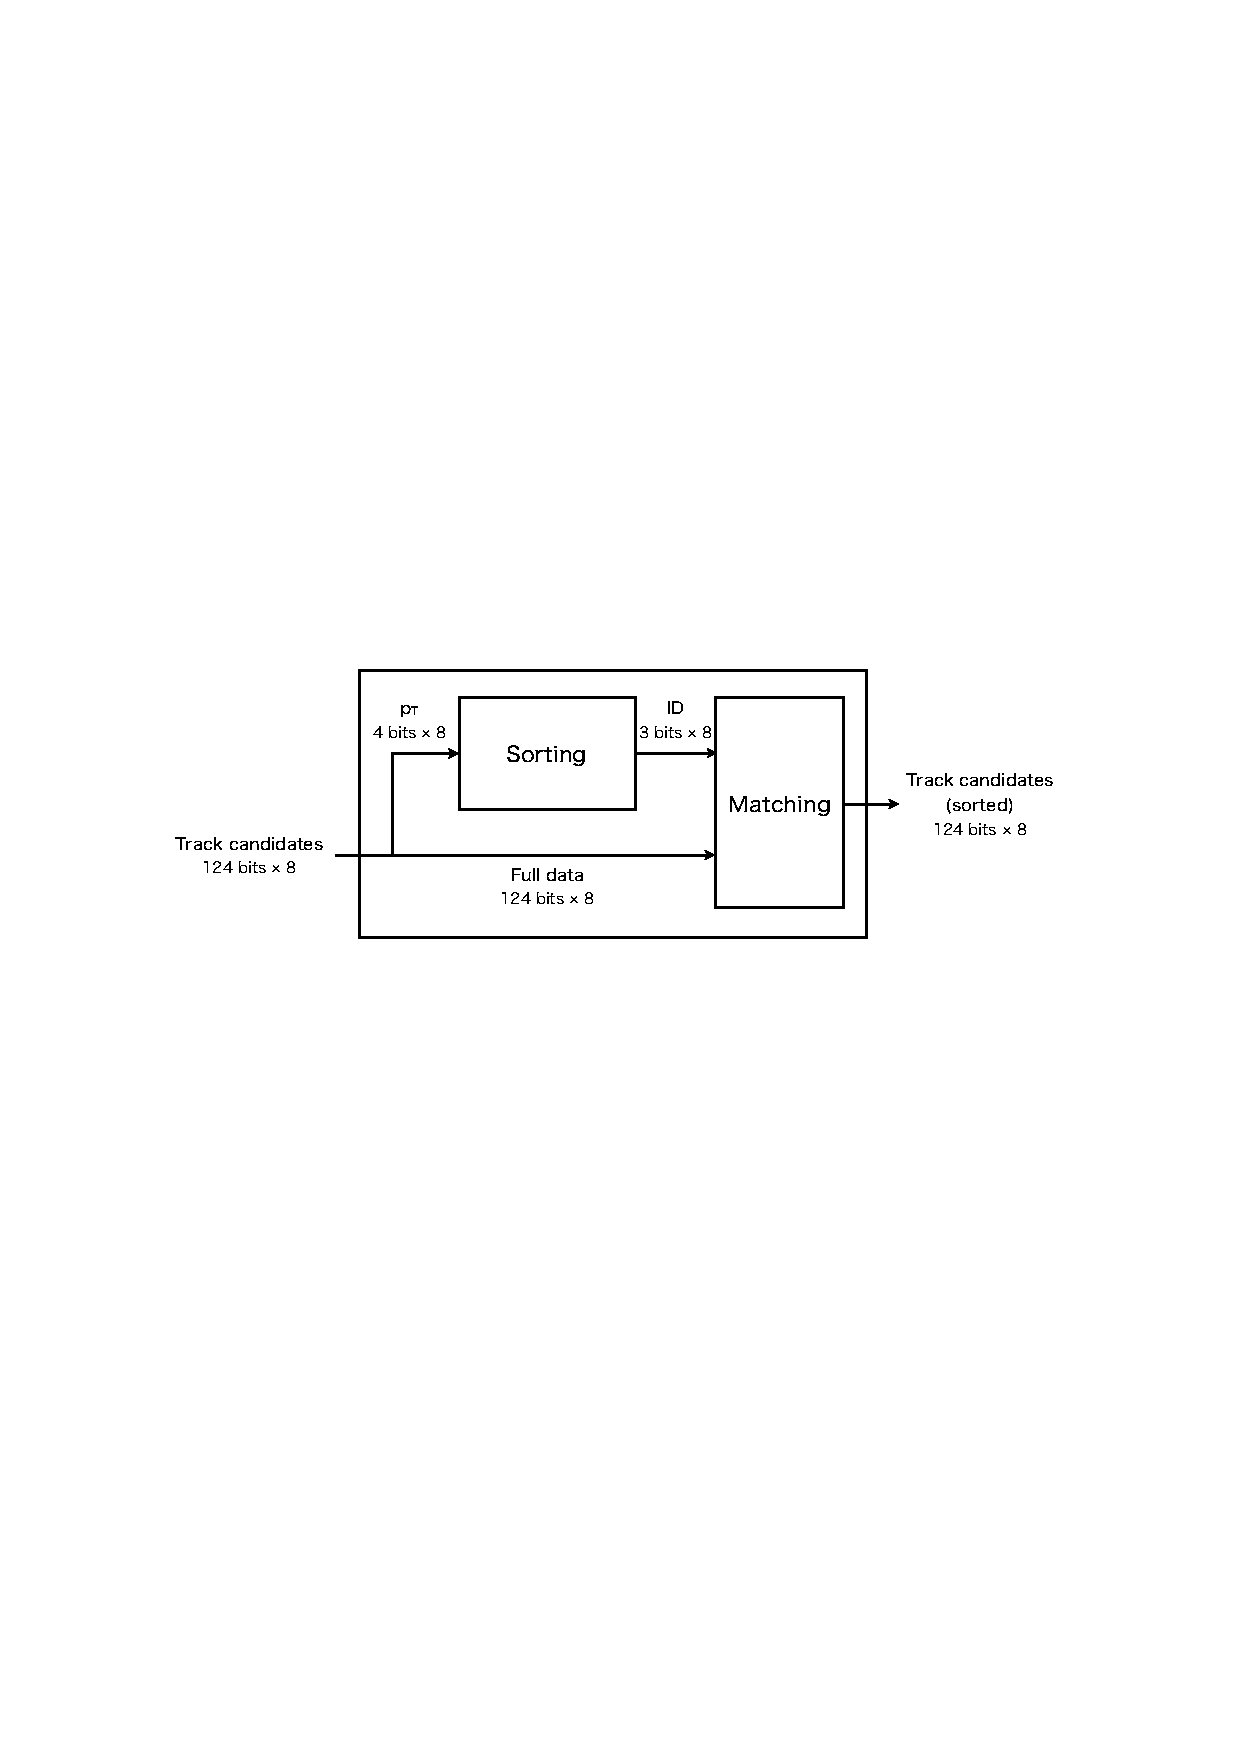
\includegraphics[width=16cm]{fig/SL/TrackSelector.pdf}
    \caption[Track Selector における選別用回路]{Track Selector における選別用回路}
    \label{TrackSelector}
\end{figure}

8-key sorting network および 16-key merging network の概要を、それぞれ図 \ref{Sortiing_8key} および図 \ref{Sorting_16} に示す。これ らの図における横線はワイヤーを表し、縦線がコンパレータを表す。左から右に向かって、それぞれのワイヤーの 比較を順番に行っていく。

\begin{figure} 
\centering
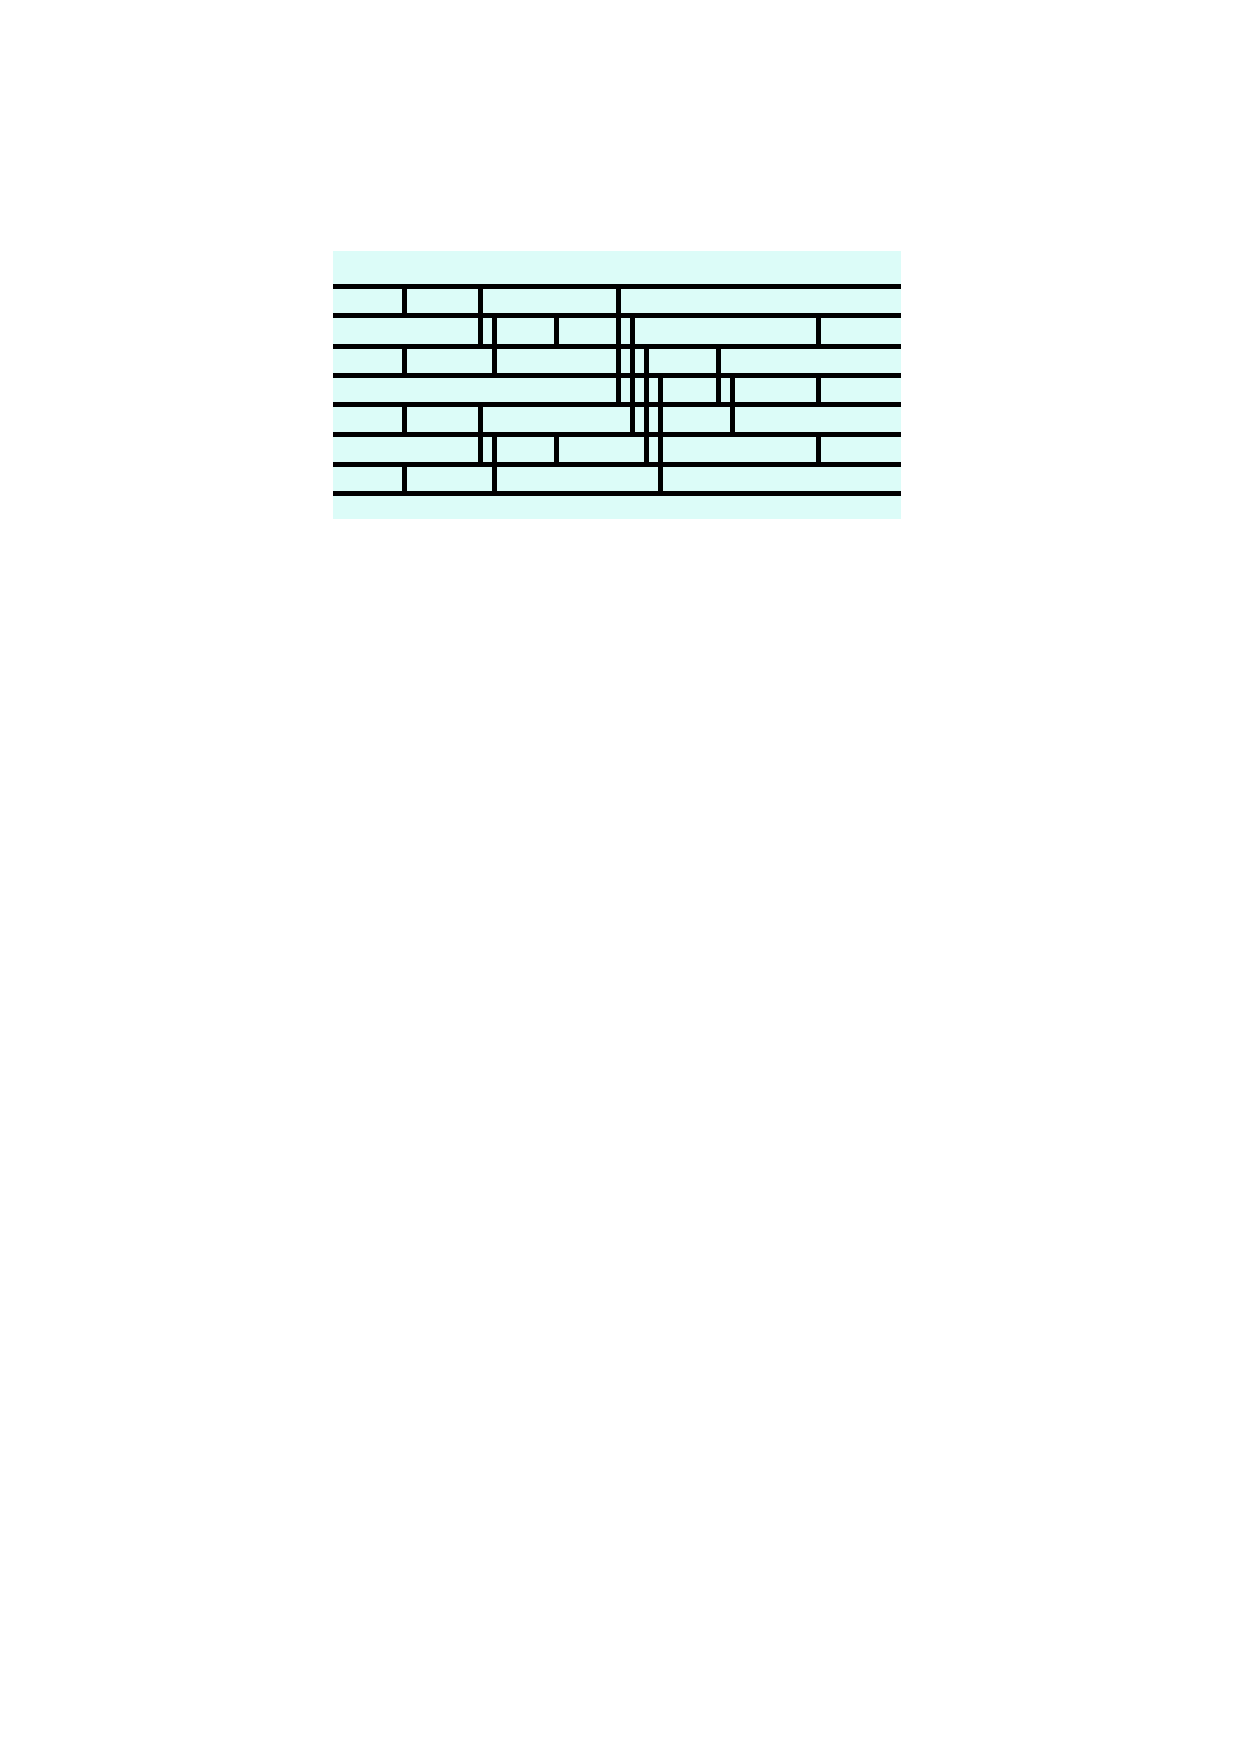
\includegraphics[width=16cm]{fig/SL/Sortiing_8key.pdf}
\caption[8-key sorting network の概要]{8-key sorting network の概要}
\label{Sortiing_8key}
\end{figure}

\begin{figure} 
\centering
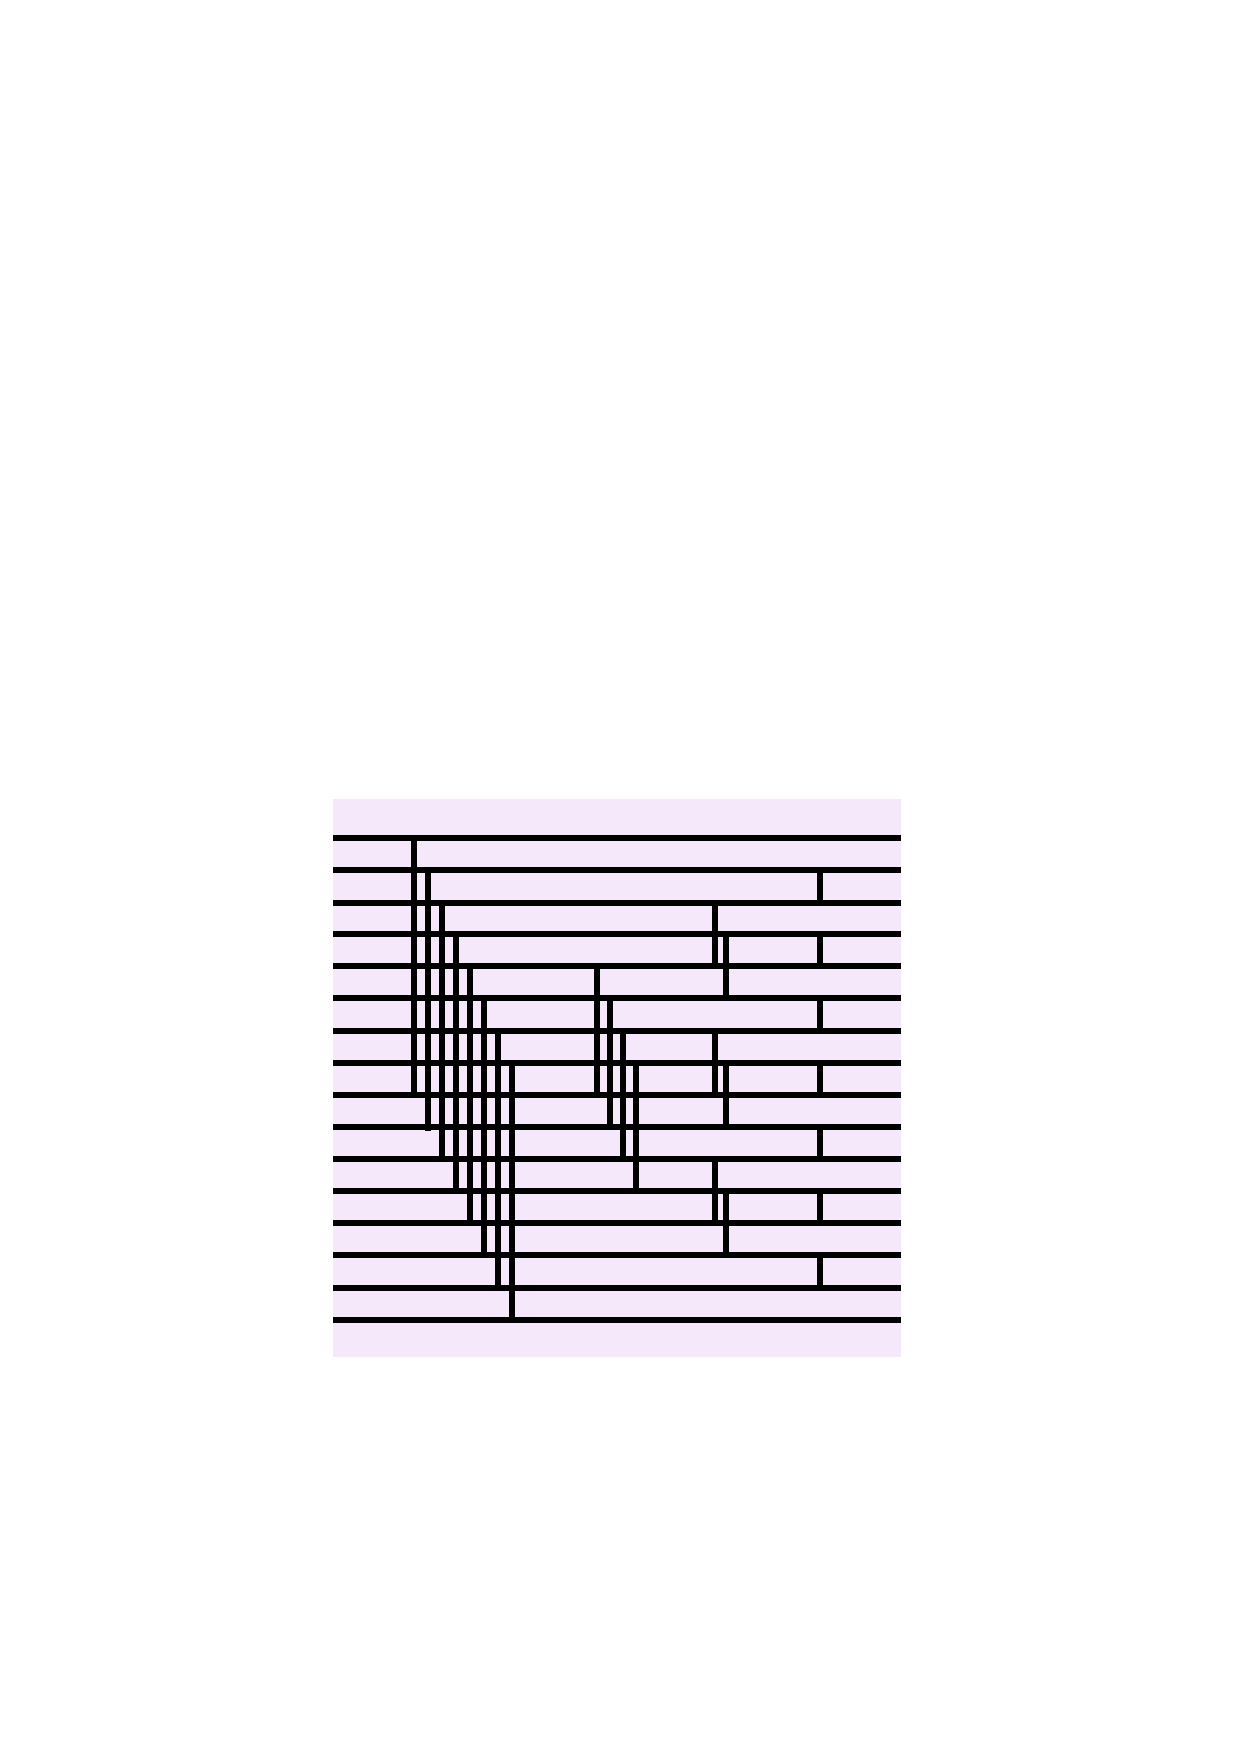
\includegraphics[width=16cm]{fig/SL/Sorting_16.pdf}
\caption[16-key merging network の概要]{16-key merging network の概要}
\label{Sorting_16}
\end{figure}


\newpage
\section{Inner Coincidenceの統合}
前節で述べたように、先行研究によりTGC BW coincidenceおよびTrack Selectorの実装が完了している。そこで本研究ではInner Coincidenceの統合を完了させ、トリガーチェーン全体を完成させる。
と、目的とするロジックをFPGAのリソース内で実現可能か、またタイミング制約を満たしつつロジックの配置ができるかといったハードウェア上の問題が生じることが懸念される。SL FPGAではこれまでのところリソースやタイミング制約に問題は発生していないが、すべてのトリガーチェーンを通した時にこれらの問題が生じないか不安視されている。大幅なロジックの変更を余儀なくされることも視野に入れて、2029年までに十分ゆとりのある今、トリガーチェーンを完成させることの意義は大きい。
そこで、本研究では先行研究で開発されたInner coincidenceを統合するため、モジュールに引き込む必要がある信号線を精査し、配線を行った。図\ref{Inner_integrate}にInner Coincidenceファームウェアの概要を示す。Inner Coincidenceは磁場内部検出器の情報と TGC BW の位置情報などをそれぞれのコインシデンスに用いるためにデコードし差分をとる “Decoder” 、それぞれの検出器とパターンマッチングをとりより精度の良い\pt を出力する”coincidence”、最終的にどの検出器とコインシデンスで得られたトリガー情報を出力するか選択する“Which-Inner”で構成される。DecoderにはTGC BWで再構成した飛跡候補の情報と、磁場内部の検出器から取得されるデータを入力する。NSW、EI、Tile、RPC coincidenceロジックは内部でLUTを用いたパターンマッチングを行なっている。そのためcoincidenceロジックにはBRAMやURAMをコンフィギュレーションするための信号を入力する。Inner Coincidenceと接続したモジュールと、各信号線のbit幅を表\ref{tab:Inner_integrate}に示す。
TGC BW coincidenceの結果としてWire Strip Coincidenceの各regionから31 bitのtrack candidateを取得する。Endcap領域を処理するSLR0、SLR2からそれぞれ4,650 bit、FW領域を処理するSLR3から992 bit、合計10,292 bitのデータをSLRを跨いで接続した。またInner CoincidenceはNSW、EI、TIle、RPCからの位置情報や角度情報を入力として利用する。しかし、磁場内部の検出器とどのようなデータを交換するか詳細が決まっておらず、インターフェイスも実装されていないため、今回はMPSoCから書き込むことができるレジスタ(Register Interface)と接続した。RAMへのLUTの書き込みは、TGC BWのLUTと同様にMPSoCをマスターにRAM Controllerを介して行う。LUTはテキストファイルに記述され、図\ref{LUT_example}に示すように、SLR Number、RAM ID、address、dataで構成される。LUTはsegment reconstruction、Wire Strip Coincidence、Inner coincidenceの各サブユニットごとに1つ用意されるため、1つのSLには合計 hoge 個のRAMが設置される。各RAMを識別するために振られているのがRAM IDで、SLRとRAM IDを指定することで書き込み動作を行うRAMを一意に決めることができる。AddressとDataはそれぞれRAM内のaddressとdataを表している。LUTを書き込むには、MPSoC上でアプリケーションを走らせテキストファイルの内容を32 bitずつRAM Controllerへ伝える。RAM ControllerはSLR、RAM ID、Address、Dataが全て揃うまで各データをバッファーする。全データが揃ったらMPSoCからactivate信号を送り、addressで指定したRAMのアドレスへdataを書き込む。そのためRAM Controllerから出力される計97 bitの信号線を接続した。Inner Coincidenceは1飛跡候補につき128 bitの情報を出力する。合計112 cand x 128 bitの信号はTrack Selectorに接続した。

\begin{figure} 
\centering
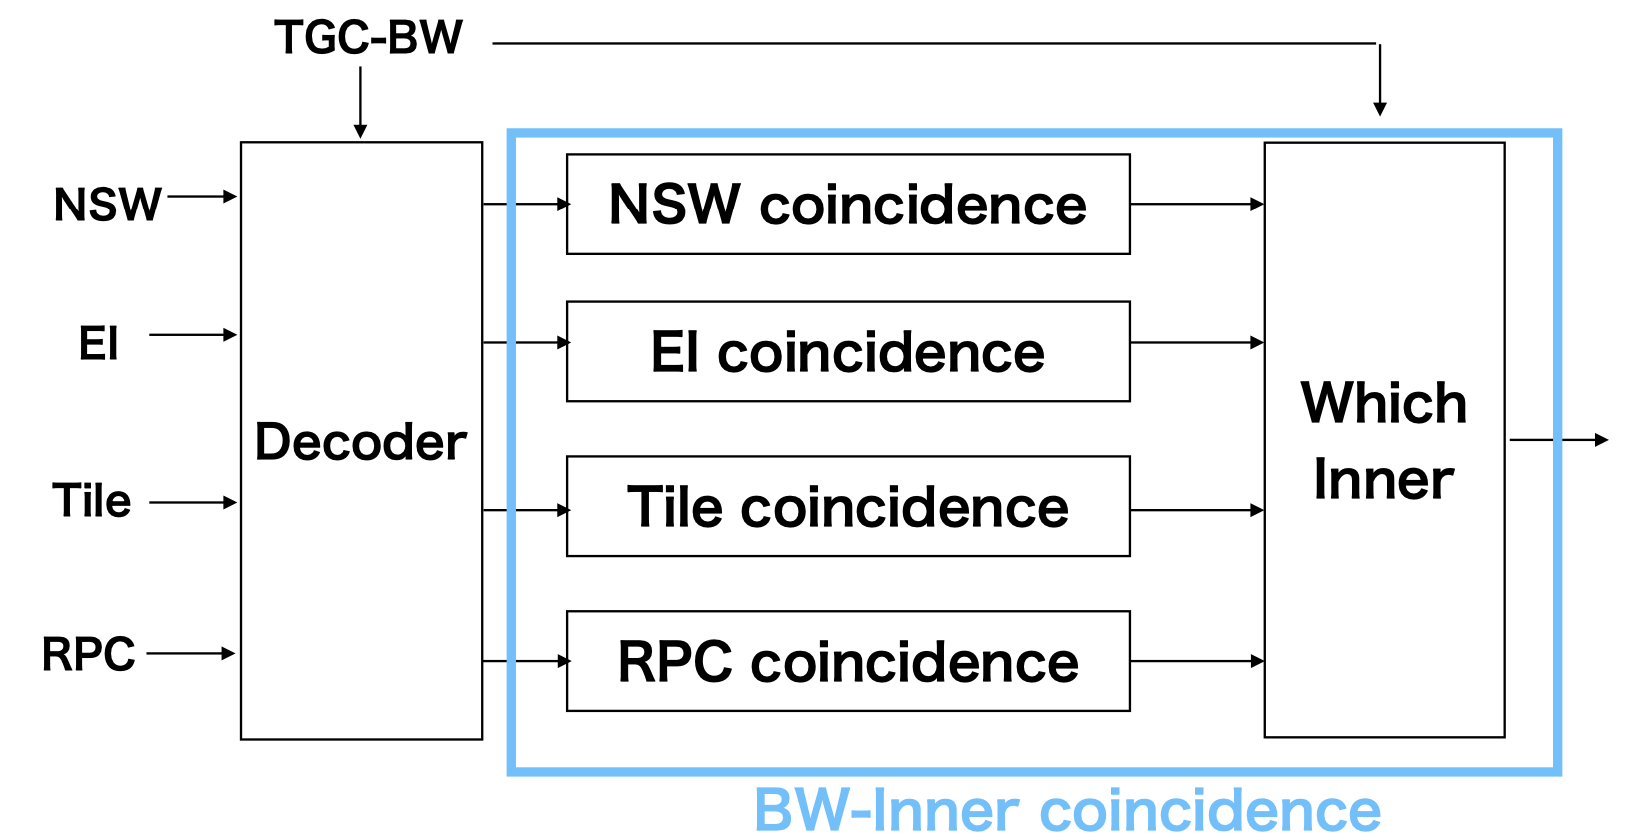
\includegraphics[width=16cm]{fig/SL/Inner_integrate.png}
\caption[Inner coincidenceファームウェアの模式図]{Inner coincidenceファームウェアの模式図\cite{mt_kobayashi}}
\label{Inner_integrate}
\end{figure}

\begin{table}[]
    \centering
    \caption{Inner Coincidenceと接続したモジュールと各信号線のbit幅}
    \label{tab:Inner_integrate}
    \begin{tabular}{|l|l|}
    \hline
    接続するモジュール                   & 信号線 (bit幅)                                                                       \\ \hline\hline
    Wire Strip Coincidence SLR0 & 8 region segment (31 bit x 22 regions) + 32 region segment (124 bit x 13 regions) \\ \hline
    Wire Strip Coincidence SLR2 & 8 region segment (31 bit x 22 regions) + 32 region segment (124 bit x 13 regions) \\ \hline
    Wire Strip Coincidence SLR3 & 32 region segment (124 bit x 8 regions)                                           \\ \hline
    Register Interface          & Tile data ( 64 )                                                                  \\ \hline
    Register Interface          & EI data ( 88 )                                                                    \\ \hline
    Register Interface          & RPC ( 96 )                                                                        \\ \hline
    Register Interface          & NSW (304 )                                                                        \\ \hline
    RAM Controller              & RAM ID (32) / wr\_addr(32) / wr\_data(32) / wr\_activate(1)                       \\ \hline
    \end{tabular}
\end{table}

\begin{figure} 
\centering
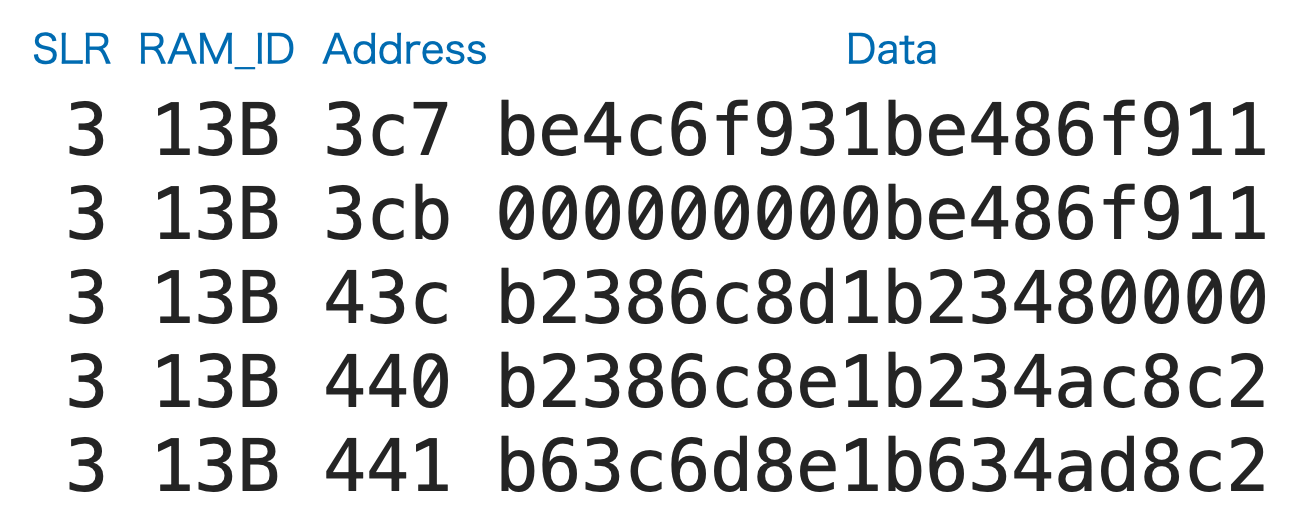
\includegraphics[width=16cm]{fig/SL/LUT_example.png}
\caption[LUTの例]{LUTの例。テキストファイルに格納され、SLR、RAM ID、Address、Dataで構成される}
\label{LUT_example}
\end{figure}

Inner Coincidenceを統合した後のデバイスのリソース使用状況を表\ref{tab:Resource_before}に示す。表中の値は、1つのSLR中のリソースに対する使用量の割合を百分率で表したものである。Totalにはトリガーロジックだけでなく、コントロール、リードアウトのロジックも含めたリソース使用状況を示している。
BRAMやURAMなどのメモリーデバイスには余裕を持って実装できている一方で、Inner Coincidenceを統合したSLR1ではConfigurable Logic Block (CLB) の使用率が100 \%に達しており、リソースが逼迫している。SLのファームウェアはまだ開発段階であり、機能が増築されていくことを考えるとリソースの削減が必要不可欠であることが判明した。
\begin{table}[]
    \centering
    \caption{Inner Coincidenceを統合した後のデバイスのリソース使用状況}
    \label{tab:Resource_before}
    \begin{tabular}{|c|c|c|c|c|c|c|c|}
    \hline
    Name                                                                        & Block                        & \begin{tabular}[c]{@{}c@{}}LUT \\ (17280000)\end{tabular} & \begin{tabular}[c]{@{}c@{}}REG \\ (34560000)\end{tabular} & \begin{tabular}[c]{@{}c@{}}CLB \\ (2160000)\end{tabular} & \begin{tabular}[c]{@{}c@{}}LUT as Memory \\ (791040)\end{tabular} & \begin{tabular}[c]{@{}c@{}}BRAM \\ (2688)\end{tabular} & \begin{tabular}[c]{@{}c@{}}URAM\\  (1280)\end{tabular} \\ \hline\hline
    \multirow{6}{*}{\begin{tabular}[c]{@{}c@{}}SLR0 \\ EC $\phi$1\end{tabular}} & Wire Station Coincidence     & 7.4                                                       & 1.48                                                      & 22.2                                                     & 0                                                                 & 0                                                      & 0                                                      \\ \cline{2-8} 
                                                                                & Strip Station Coincidence    & 0                                                         & 0.2                                                       & 0.96                                                     & 0                                                                 & 0                                                      & 0                                                      \\ \cline{2-8} 
                                                                                & Wire Segment Reconstruction  & 16.28                                                     & 2.96                                                      & 28.12                                                    & 0                                                                 & 0                                                      & 45.88                                                  \\ \cline{2-8} 
                                                                                & Strip Segment Reconstruction & 6.24                                                      & 3.08                                                      & 11.04                                                    & 0.08                                                              & 0                                                      & 2.43                                                   \\ \cline{2-8} 
                                                                                & Wire Strip Coincidence       & 3.56                                                      & 3.76                                                      & 14.56                                                    & 0                                                                 & 37.52                                                  & 0                                                      \\ \cline{2-8} 
                                                                                & Total                        & 58.24                                                     & 31.04                                                     & 95.28                                                    & 1.08                                                              & 73.68                                                  & 51.56                                                  \\ \hline\hline
    \multirow{3}{*}{SLR1}                                                       & Inner Coincidence            & 67.8                                                      & 19                                                        & 83.64                                                    & 3                                                                 & 28.88                                                  & 50                                                     \\ \cline{2-8} 
                                                                                & Track Selector               & 15.4                                                      & 1.76                                                      & 17.72                                                    & 0                                                                 & 0                                                      & 0                                                      \\ \cline{2-8} 
                                                                                & Total                        & 87.16                                                     & 45.24                                                     & 100                                                      & 3                                                                 & 28.88                                                  & 50                                                     \\ \hline\hline
    \multirow{6}{*}{\begin{tabular}[c]{@{}c@{}}SLR2 \\ EC $\phi$1\end{tabular}} & Wire Station Coincidence     & 7.4                                                       & 1.48                                                      & 22.2                                                     & 0                                                                 & 0                                                      & 0                                                      \\ \cline{2-8} 
                                                                                & Strip Station Coincidence    & 0                                                         & 0.2                                                       & 0.96                                                     & 0                                                                 & 0                                                      & 0                                                      \\ \cline{2-8} 
                                                                                & Wire Segment Reconstruction  & 16.28                                                     & 2.96                                                      & 28.12                                                    & 0                                                                 & 0                                                      & 45.88                                                  \\ \cline{2-8} 
                                                                                & Strip Segment Reconstruction & 6.24                                                      & 3.08                                                      & 11.04                                                    & 0.08                                                              & 0                                                      & 2.43                                                   \\ \cline{2-8} 
                                                                                & Wire Strip Coincidence       & 3.56                                                      & 3.76                                                      & 14.56                                                    & 0                                                                 & 37.52                                                  & 0                                                      \\ \cline{2-8} 
                                                                                & Total                        & 58.24                                                     & 31.04                                                     & 95.28                                                    & 1.08                                                              & 73.68                                                  & 51.56                                                  \\ \hline\hline
    \multirow{6}{*}{\begin{tabular}[c]{@{}c@{}}SLR3 \\ FW\end{tabular}}         & Wire Station Coincidence     & 3.84                                                      & 0.64                                                      & 8.96                                                     & 0                                                                 & 0                                                      & 0                                                      \\ \cline{2-8} 
                                                                                & Strip Station Coincidence    & 0                                                         & 0.04                                                      & 0.16                                                     & 0                                                                 & 0                                                      & 0                                                      \\ \cline{2-8} 
                                                                                & Wire Segment Reconstruction  & 6.4                                                       & 1.28                                                      & 9.6                                                      & 0                                                                 & 0                                                      & 19.84                                                  \\ \cline{2-8} 
                                                                                & Strip Segment Reconstruction & 1.24                                                      & 0.6                                                       & 2.52                                                     & 0.04                                                              & 0                                                      & 1.24                                                   \\ \cline{2-8} 
                                                                                & Wire Strip Coincidence       & 1.52                                                      & 1.6                                                       & 5.36                                                     & 0                                                                 & 14.28                                                  & 0                                                      \\ \cline{2-8} 
                                                                                & Total                        & 25.84                                                     & 15.88                                                     & 52.04                                                    & 0.48                                                              & 32.52                                                  & 20.32                                                  \\ \hline
    \end{tabular}
\end{table}

タイミングの解析の結果を表\ref{tab:timing_before}に示す。
Setup解析、Hold解析どちらにおいてもタイミング違反 (タイミングバイオレーション) が発生した。本研究では特に、Total Negative Slack (TNS) をタイミング違反の定量化に利用する。TNSとは、FPGA内に含まれる全てのフリップフロップパス間のネガティブスラックを足し上げたもので、どれだけタイミング深刻なタイミング違反かということと (Worst Negative Slack , WNS) と、どれだけ広範囲にタイミング違反が生じているか ( Number of Failing EndPoints )どちらにも相関を持つ値となっている。タイミング違反が発生した場合には負の値をとる。タイミングバイオレーションが生じている場合、ファームウェアの正常動作は保証されないため、これに関しても改善が必要である。
\begin{table}[]
    \centering
    \caption{Inner Coincidence統合後のタイミング解析の結果}
    \label{tab:timing_before}
    \begin{tabular}{|c|c|c|}
    \hline
    Name                                                    & Setup         & Hold        \\ \hline\hline
    Worst Negative Slack (WNS) / Worst Hold Slack (WHS)     & -8.616 ns     & -0.256 ns   \\ \hline
    Number of Failing Endpoints / Total Number of Endpoints & 59 K / 1911 K & 9K / 1911 K \\ \hline
    Total Negative Slack (TNS) / Total Hold slack           & -126, 297 ns  & -388 ns     \\ \hline
    \end{tabular}
\end{table}

\section{タイミングバイオレーションへの対処}
本節ではInner Coincidenceを統合したことにより生じたタイミングバイオレーションを解決するために行った2つの最適化について説明する。いずれも、FPGAで実現される論理自体に変更を加えることなく、リソースの使い方を最適化したものであり、トリガーロジックの性能に影響を与えるものではない。

\subsection{シフトレジスタ実装方法の最適化}
タイミングバイオレーション問題の解決に向けて、まずシフトレジスターの実装方法を検討した。
一般に、FPGAでタイミング違反が生じた場合、2つのフリップフロップ間にシフトレジスターを挟む処理が行われる。これは、回路の大規模化に伴ってフリップフロップが離れた位置に配置された場合でも、シフトレジスたを挟むことで、フリップフロップ間の距離が短くなりタイミング制約を緩和することができるからである。この目的で挿入されるシフトレジスタをパイプラインレジスタと呼ぶ。SL FPGAでもこれまでタイミング違反が生じた場合に、この処置がとられて来た。たとえば、Wire Station CoincidenceとWire Segment Reconstructionの間で2段、Wire Segment ReconstructionとWire Strip Coincidenceの間で2段のパイプラインレジスタが挿入されている。

ところで、UltraScale+ FPGAではシフトレジスタを実装するのに2種類のプリミティブ\footnote{FPGAの最小構成要素。FPGAの論理回路はプリミティブの組み合わせで構成される。代表的にはLUT、Flip Flop、RAMなどがある。目的の論理回路を実現するのにどのプリミティブを利用し、FPGA内のどこに配置するかは”Vivado”ソフトウェアで自動で行われる。}が用意されている。それぞれの概要を図\ref{SL_ShiftRegister}に示す。1つ目はD Flip-Flop with Clock Enable and Synchronous Reset (FDRE)と呼ばれる基本的なフリップフロップである。1つのFDREは1 bitのデータを保持するため、width n, depth mのシフトレジスタを実装するにはn x m個のFDREが必要となる。2つ目はShift Register LUT (SRL)と呼ばれる、メモリー用のLUTである。最大のdepthが16のもの(SRL16E) と32 (SRLC32E)のものが存在し、同様のシフトレジスターをSRLC32Eで実現しようとすると n x (m/32)個プリミティブを使用する。

\begin{figure}
\begin{minipage}[b]{.5\linewidth}
\centering
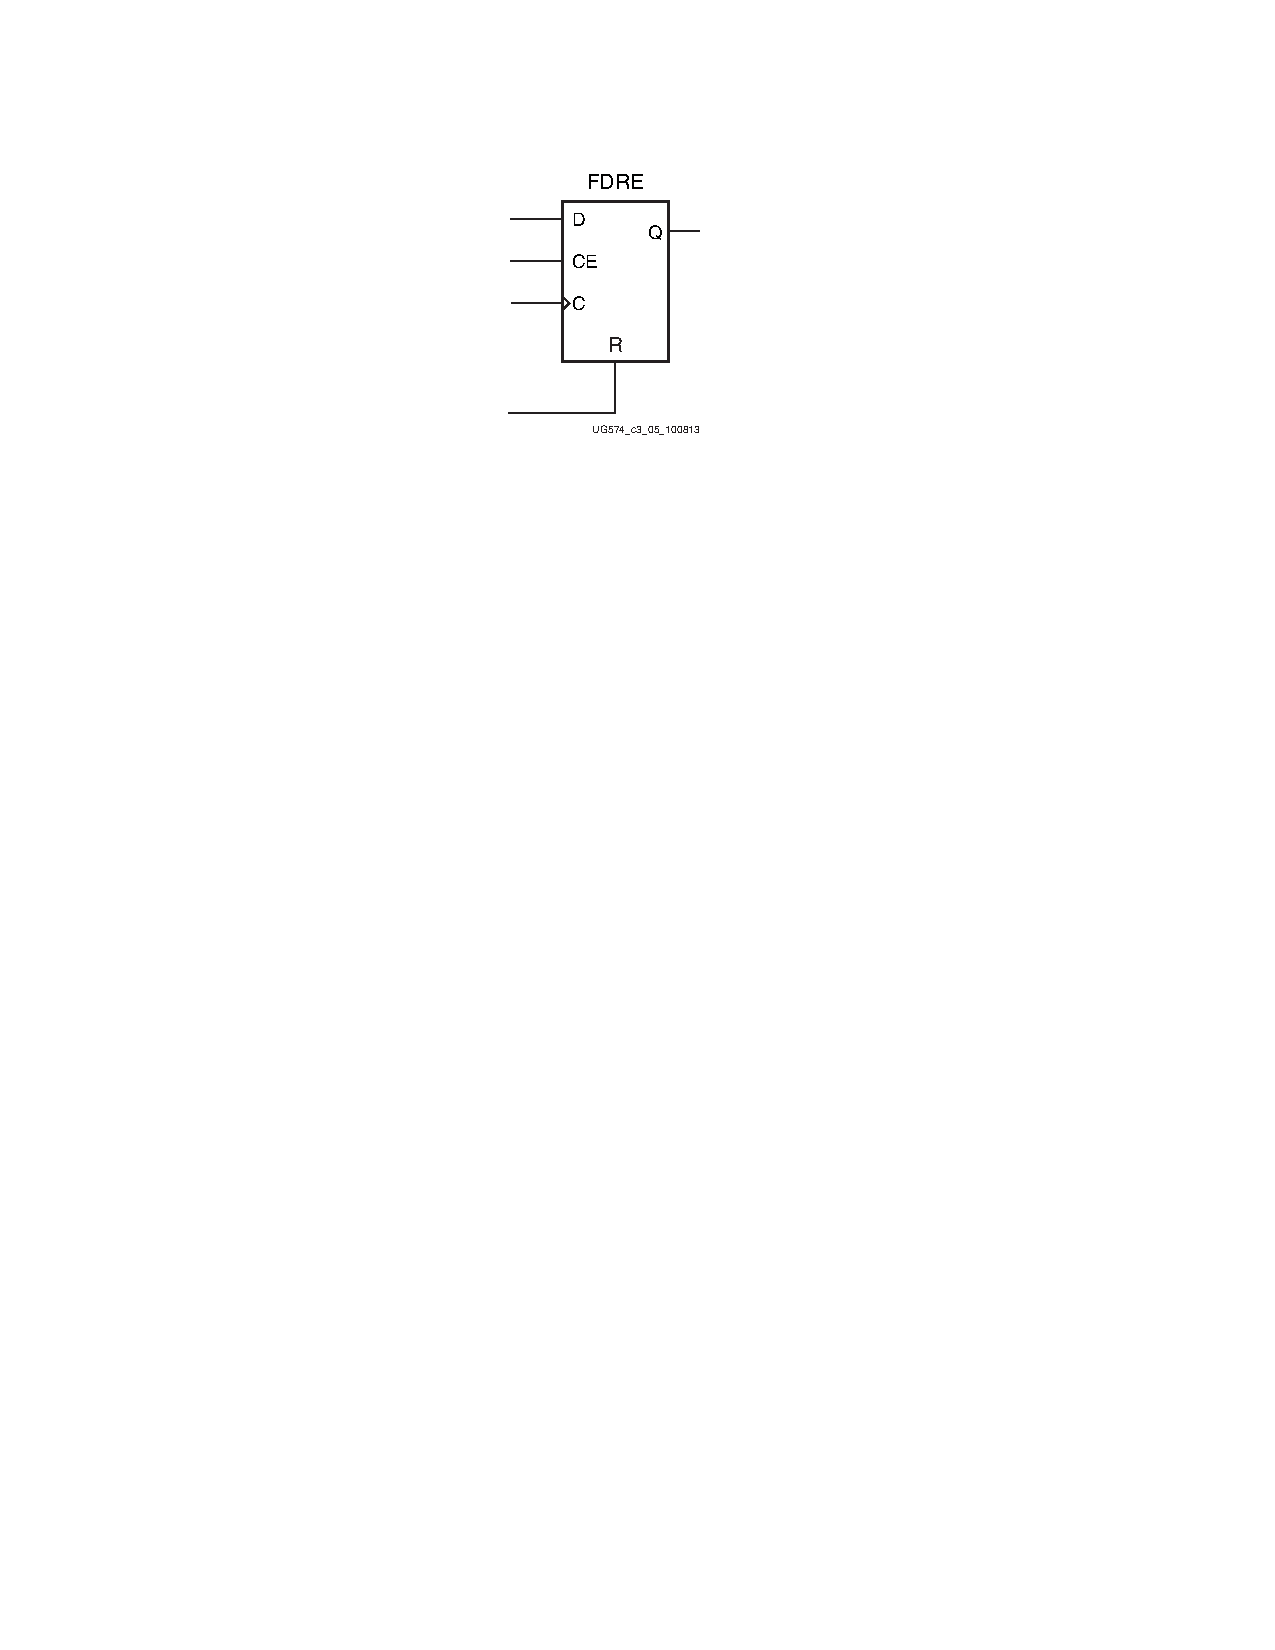
\includegraphics[height=5cm]{fig/SL/FDRE.pdf}
\subcaption{FERE Primitiveのロジックブロック}
\end{minipage}%
\begin{minipage}[b]{.5\linewidth}
\centering
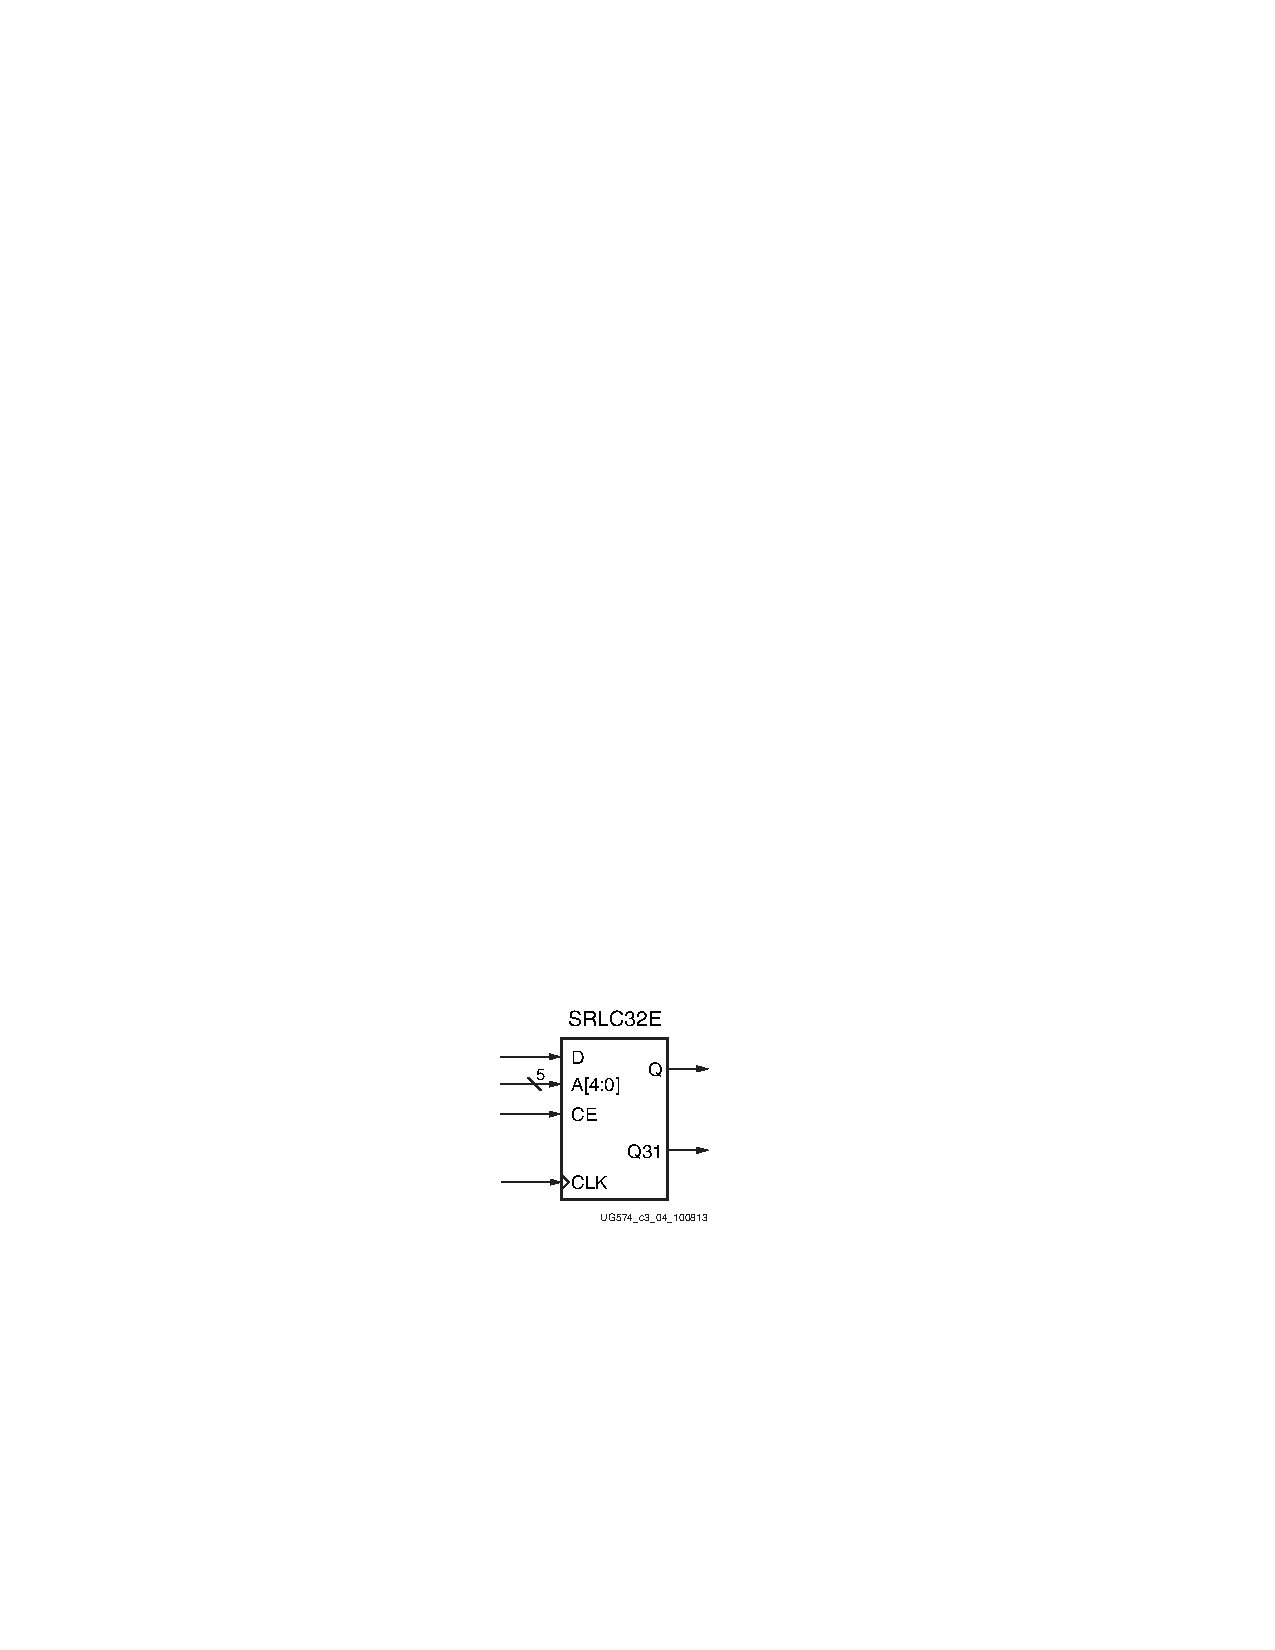
\includegraphics[height=5cm]{fig/SL/SRLC32E.pdf}
\subcaption{SRLC32E Primitiveのロジックブロック}
\end{minipage}%
\caption[シフトレジスタを構成するプリミティブ]{異シフトレジスタを構成するプリミティブ\cite{UltraScale_Architecture}}
\label{SL_ShiftRegister}
\end{figure}

これまでSL FPGAではパイプラインレジスタを実現するのにFDREのみを利用していた。これは一連のシフトレジスタがが1つのSRLタイルに配置されると、ロジックとロジックを繋ぐ中継点の役割を果たさず、タイミング制約を緩和するという本来の役割を果たさなくなると考えられていたからである。しかし、ロジックが大規模になり、基本的なプリミティブであるFDREの使用量が増えてくるとFPGA内に密集が発生し、逆に適切な位置にパイプラインレジスタを配置できなくなることも考えられる。そこで、本研究ではFDREに加えてSRLも利用してimplemetationを行い、どちらの方がタイミング制約の緩和に有効な実装方法か調査した。

図\ref{SRL_FDRE}にSLR0のプリミティブ使用状況を示す。図の黄色のcellがSLR0内のパイプラインレジスタの実装に利用されているプリミティブである。FDREのみを利用した場合、パイプラインレジスタはFDRE 50 K個を用いて実装されている。一方SRLも利用した場合、パイプラインレジスタはSRL 6K、FDRE 6K個を利用して実装される。
図\ref{}に変更前後におけるファームウェア全体でのネガティブスラック発生状況、表\ref{}にタイミング解析の結果を示す。SRLを利用することで、TNSは-126297.769 ns から -7903.744 nsに約1/16に削減された。この結果は、SRLを使うと、フリップフロップ間の距離が遠いところには適切にパイプラインを設置し、逆に近いところでは数段のパイプラインをまとめてSRLに実装するなど、より柔軟なロジックの配置が実現したことによるものと考えられる。
しかし依然としてタイミングバイオレーションは解決しておらず、さらなる改善が求められる。

\begin{figure} 
\centering
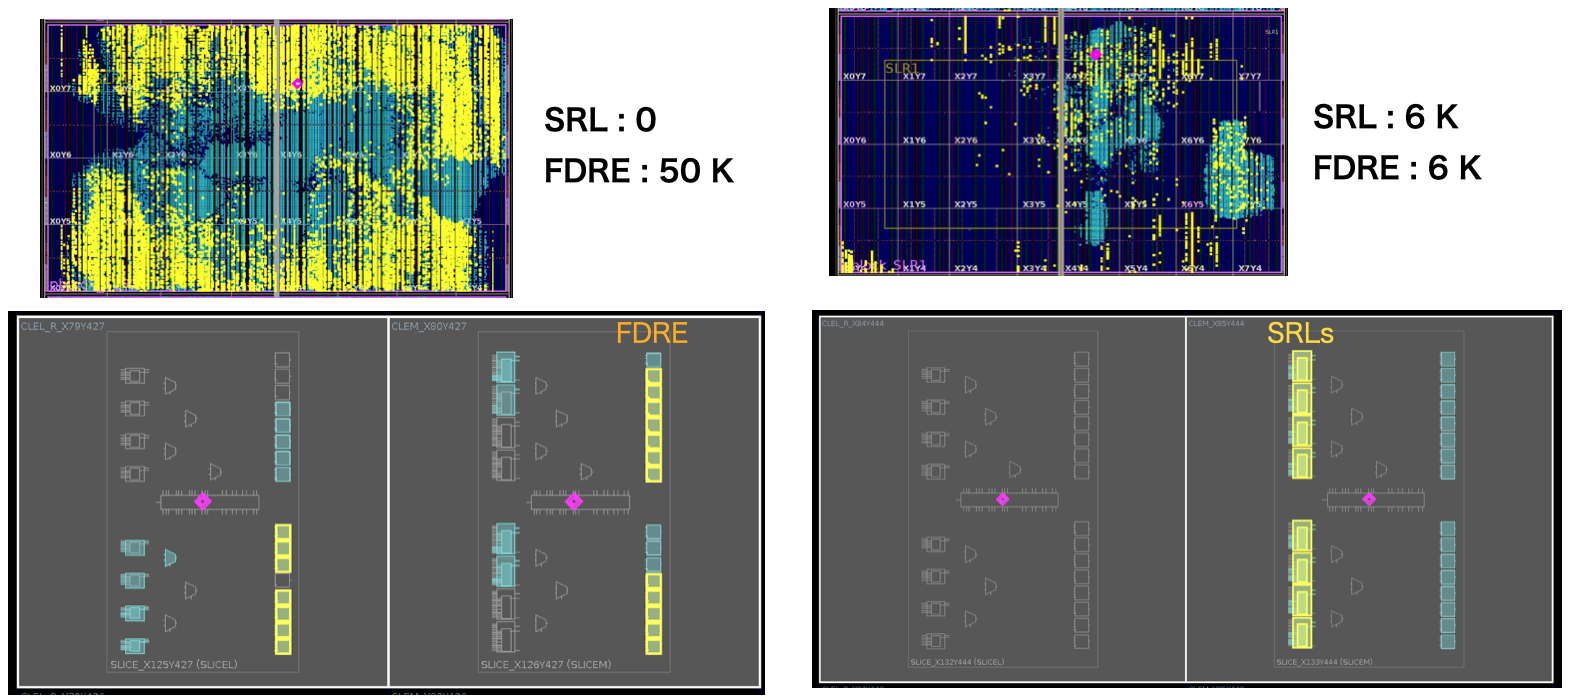
\includegraphics[width=16cm]{fig/SL/SRL_FERE.png}
\caption[SRLを利用する場合と利用しない場合におけるリソース使用状況の比較]{SRLを利用する場合と利用しない場合におけるリソース使用状況の比較}
\label{SRL_FDRE}
\end{figure}


\subsection{Track Selectorの最適化}
モジュールごとのネガティブスラックの量をみると、全体の50 \%以上がTrack Selectorで発生しており、トリガーチェーンをタイミング制約を満たして完成させるにはこれの最適化が必要である。そこで本研究ではTrack Selectorにかけるレイテンシーを160 MHz 1チック分増やす代わりに、ソーティングロジックの簡略化を行い、タイミング制約の緩和を図った。
従来のロジックと変更後のロジックの概念図を図\ref{}に示す。Track SelectorはInner Coincidenceから出力された最大128個のミューオン飛跡候補から、\pt の大きいものを8個選び出すものである。1つのミューオン候補に対して124 bitの情報が用意される。128個の飛跡候補は160 MHzの1チックごとに1 vs 1で\pt 比較が行われ、合計4チックで8候補まで絞り込まれる。従来のロジックではこのソーティングのロジックにおいて124 bit $\times$ 128 候補のデータを並列に並べた上で、124 bitのデータ同士を並び替えていた。これに対し、変更後のロジックではInner Coincidenceから出力される1候補あたり124 bitのデータのうち、ソーティングに利用する\pt 5 bitの情報だけを取り出し並び替えを行い、そのほかのデータは128個の飛跡候補を識別する 7 bit のIDと共にBRAMに格納しておく。ソーティングが完了し8個の飛跡候補が選ばれたら、そのIDを用いてBRAMからデータを取り出す。
この方法では、ソーティングの後BRAMからデータを取り出すのに160 MHz 1チック分レイテンシーが余計にかかってしまうが、ソーティング必要なデータ量を124 bit $\times$ 128 候補から5 bit $\times$ 128 候補に削減することができる。これにより、FPGAで配線する必要のあるプリミティブを大幅に減らすことができ、タイミング制約の緩和が期待される。

図\ref{SL_Metrics}および表\ref{tab:timing_before_after}に最適化前後のタイミング解析の結果をまとめる。シフトレジスタの最適化後にあった-7903.744 nsのTNSは0になっており、タイミングバイオレーションを解決することができた。


\begin{table}[]
    \centering
    \caption{Track Selectorの最適化前後のタイミング解析の結果}
    \label{tab:timing_before_after}
    \begin{tabular}{|c||cc||cc||cc|}
    \hline
    \multirow{2}{*}{Name}                                                                              & \multicolumn{2}{c||}{最適化前}                        & \multicolumn{2}{c||}{シフトレジスタ最適化}                 & \multicolumn{2}{c||}{Track Selector最適化}      \\ \cline{2-7}
                                                                                                       & \multicolumn{1}{c|}{Setup}         & Hold        & \multicolumn{1}{c|}{Setup}         & Hold       & \multicolumn{1}{c|}{Setup}      & Hold      \\ \hline
    Worst  Slack                                                                                       & \multicolumn{1}{c|}{-8.616 ns}     & -0.256 ns   & \multicolumn{1}{c|}{- 1.164 ns}    & 0          & \multicolumn{1}{c|}{0}          & 0         \\ \hline
    \begin{tabular}[c]{@{}c@{}}Number of Failing Endpoints / \\ Total Number of Endpoints\end{tabular} & \multicolumn{1}{c|}{59 K / 1911 K} & 9K / 1911 K & \multicolumn{1}{c|}{14 K / 1643 K} & 0 / 1643 K & \multicolumn{1}{c|}{0 / 1716 K} & 0 /1716 K \\ \hline
    Total Slack                                                                                        & \multicolumn{1}{c|}{-126, 297 ns}  & -388 ns     & \multicolumn{1}{c|}{- 7903.744}    & 0          & \multicolumn{1}{c|}{0}          & 0         \\ \hline
    \end{tabular}
\end{table}

\begin{figure}
\begin{minipage}[b]{.33\linewidth}
\centering
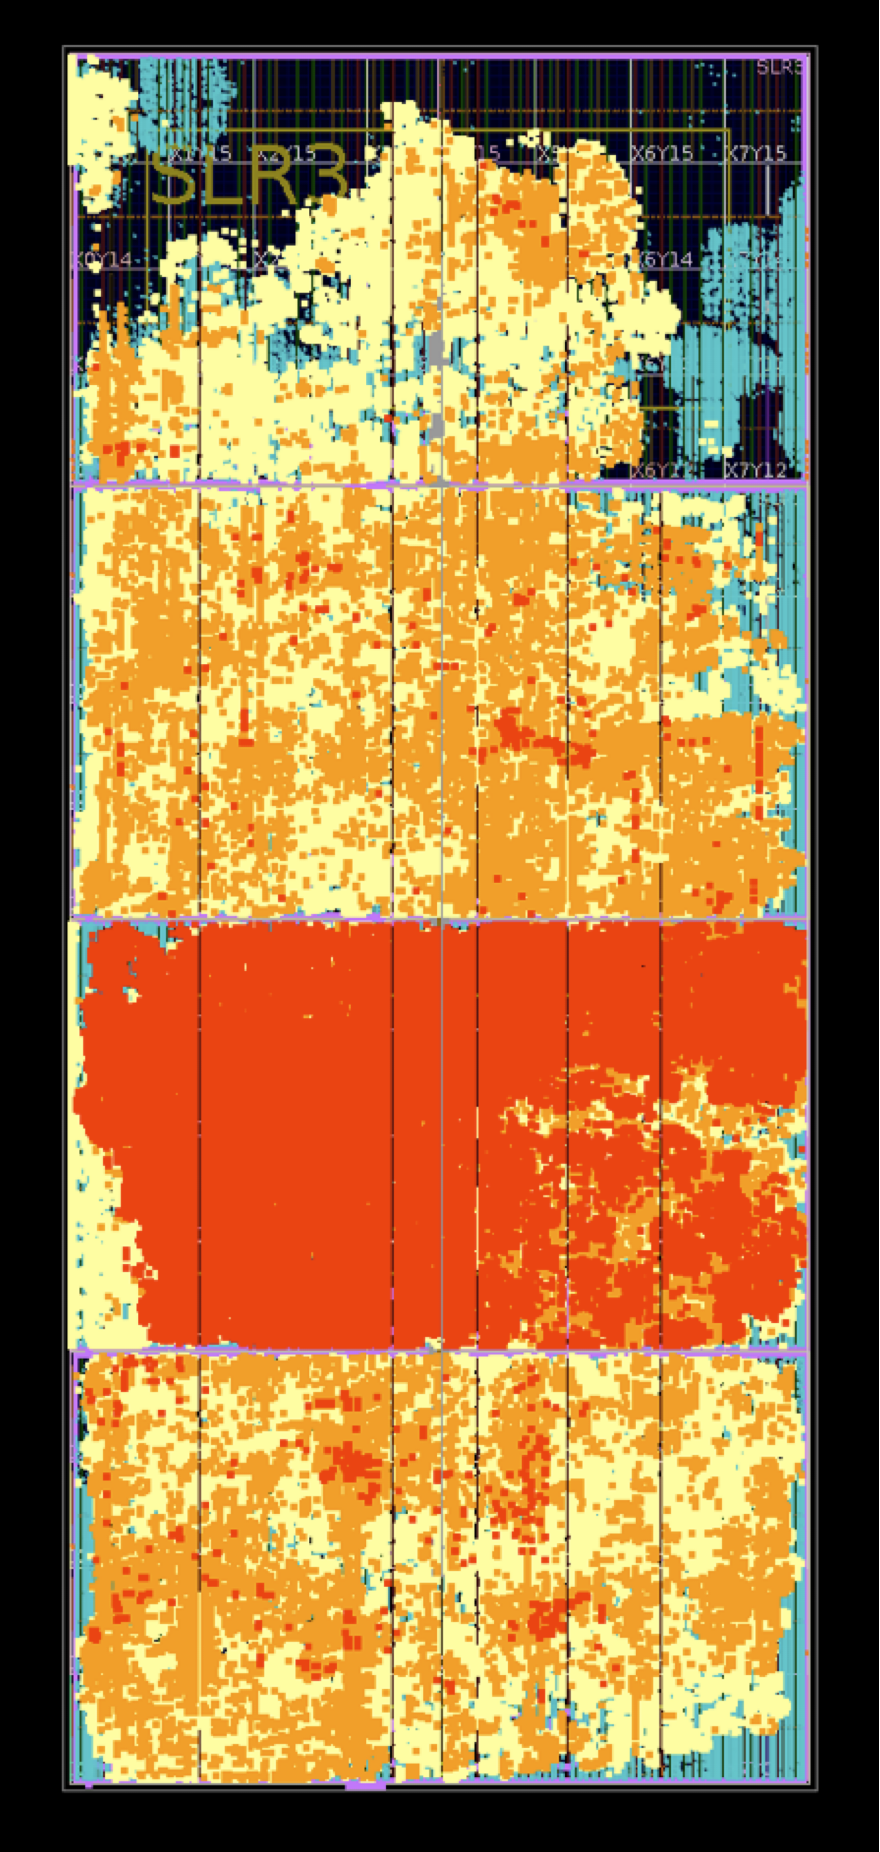
\includegraphics[height=12cm]{fig/SL/Metrics_before.png}
\subcaption{最適化前}
\end{minipage}%
\begin{minipage}[b]{.33\linewidth}
\centering
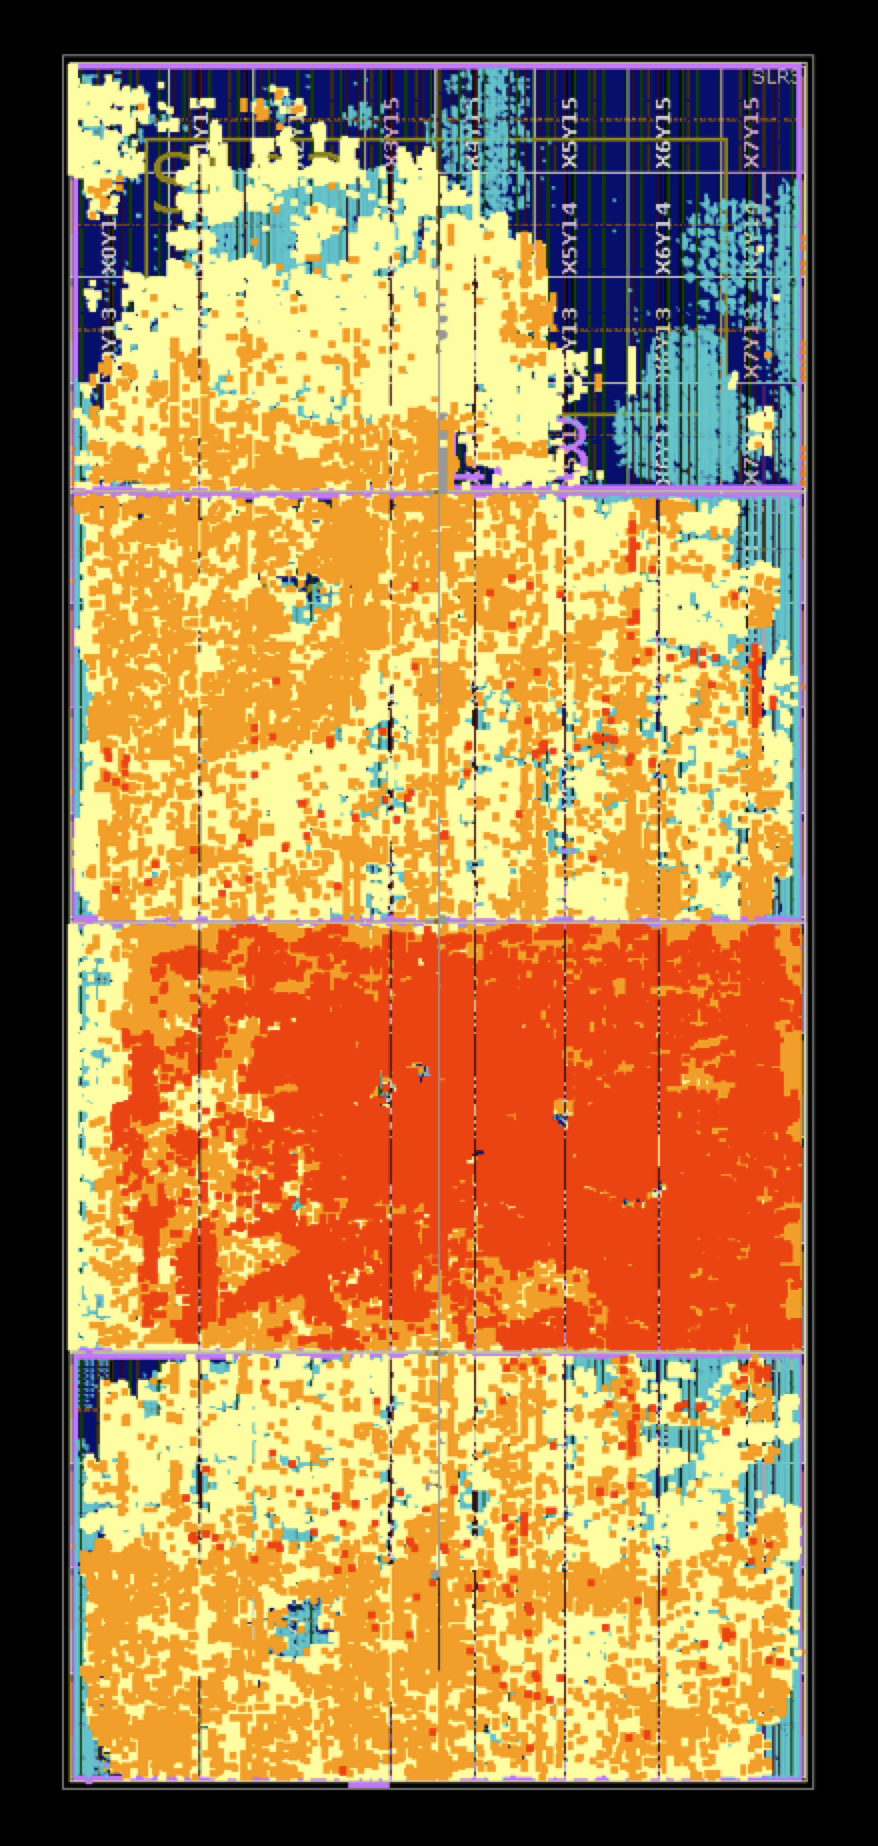
\includegraphics[height=12cm]{fig/SL/Metrics_shiftreg.png}
\subcaption{シフトレジスタ最適化後}
\end{minipage}%
\begin{minipage}[b]{.33\linewidth}
\centering
\includegraphics[height=12cm]{fig/SL/Metrics_trackselector.png}
\subcaption{Track Selector最適化後}
\end{minipage}%
\caption[]{最適化前後のネガティブスラック発生状況。赤色のセルがネガティブスラックが発生している領域を示す。オレンジ、黄色、白色の順に正のスラックが大きい。シフトレジスタの最適化とTrack Selectorの最適化を経て、タイミングバイオレーションを解決することができた。}
\label{SL_Metrics}
\end{figure}

また、最適化後のリソース使用状況を図\ref{tab:Resource_after}に示す。

\begin{table}[]
    \centering
    \caption{最適化後のデバイスのリソース使用状況}
    \label{tab:Resource_after}
    \begin{tabular}{|c|c|c|c|c|c|c|c|}
    \hline
    Name                                                                        & Block                        & \begin{tabular}[c]{@{}c@{}}LUT \\ (17280000)\end{tabular} & \begin{tabular}[c]{@{}c@{}}REG \\ (34560000)\end{tabular} & \begin{tabular}[c]{@{}c@{}}CLB \\ (2160000)\end{tabular} & \begin{tabular}[c]{@{}c@{}}LUT as Memory \\ (791040)\end{tabular} & \begin{tabular}[c]{@{}c@{}}BRAM \\ (2688)\end{tabular} & \begin{tabular}[c]{@{}c@{}}URAM\\  (1280)\end{tabular} \\ \hline\hline
    \multirow{6}{*}{\begin{tabular}[c]{@{}c@{}}SLR0 \\ EC $\phi$1\end{tabular}} & Wire Station Coincidence     & 7.4                                                       & 1.48                                                      & 22.2                                                     & 0                                                                 & 0                                                      & 0                                                      \\ \cline{2-8} 
                                                                                & Strip Station Coincidence    & 0                                                         & 0.2                                                       & 0.96                                                     & 0                                                                 & 0                                                      & 0                                                      \\ \cline{2-8} 
                                                                                & Wire Segment Reconstruction  & 16.28                                                     & 2.96                                                      & 28.12                                                    & 0                                                                 & 0                                                      & 45.88                                                  \\ \cline{2-8} 
                                                                                & Strip Segment Reconstruction & 6.24                                                      & 3.08                                                      & 11.04                                                    & 0.08                                                              & 0                                                      & 2.43                                                   \\ \cline{2-8} 
                                                                                & Wire Strip Coincidence       & 3.56                                                      & 3.76                                                      & 14.56                                                    & 0                                                                 & 37.52                                                  & 0                                                      \\ \cline{2-8} 
                                                                                & Total                        & 58.24                                                     & 31.04                                                     & 95.28                                                    & 1.08                                                              & 73.68                                                  & 51.56                                                  \\ \hline\hline
    \multirow{3}{*}{SLR1}                                                       & Inner Coincidence            & 67.8                                                      & 19                                                        & 83.64                                                    & 3                                                                 & 28.88                                                  & 50                                                     \\ \cline{2-8} 
                                                                                & Track Selector               & 15.4                                                      & 1.76                                                      & 17.72                                                    & 0                                                                 & 0                                                      & 0                                                      \\ \cline{2-8} 
                                                                                & Total                        & 87.16                                                     & 45.24                                                     & 100                                                      & 3                                                                 & 28.88                                                  & 50                                                     \\ \hline\hline
    \multirow{6}{*}{\begin{tabular}[c]{@{}c@{}}SLR2 \\ EC $\phi$1\end{tabular}} & Wire Station Coincidence     & 7.4                                                       & 1.48                                                      & 22.2                                                     & 0                                                                 & 0                                                      & 0                                                      \\ \cline{2-8} 
                                                                                & Strip Station Coincidence    & 0                                                         & 0.2                                                       & 0.96                                                     & 0                                                                 & 0                                                      & 0                                                      \\ \cline{2-8} 
                                                                                & Wire Segment Reconstruction  & 16.28                                                     & 2.96                                                      & 28.12                                                    & 0                                                                 & 0                                                      & 45.88                                                  \\ \cline{2-8} 
                                                                                & Strip Segment Reconstruction & 6.24                                                      & 3.08                                                      & 11.04                                                    & 0.08                                                              & 0                                                      & 2.43                                                   \\ \cline{2-8} 
                                                                                & Wire Strip Coincidence       & 3.56                                                      & 3.76                                                      & 14.56                                                    & 0                                                                 & 37.52                                                  & 0                                                      \\ \cline{2-8} 
                                                                                & Total                        & 58.24                                                     & 31.04                                                     & 95.28                                                    & 1.08                                                              & 73.68                                                  & 51.56                                                  \\ \hline\hline
    \multirow{6}{*}{\begin{tabular}[c]{@{}c@{}}SLR3 \\ FW\end{tabular}}         & Wire Station Coincidence     & 3.84                                                      & 0.64                                                      & 8.96                                                     & 0                                                                 & 0                                                      & 0                                                      \\ \cline{2-8} 
                                                                                & Strip Station Coincidence    & 0                                                         & 0.04                                                      & 0.16                                                     & 0                                                                 & 0                                                      & 0                                                      \\ \cline{2-8} 
                                                                                & Wire Segment Reconstruction  & 6.4                                                       & 1.28                                                      & 9.6                                                      & 0                                                                 & 0                                                      & 19.84                                                  \\ \cline{2-8} 
                                                                                & Strip Segment Reconstruction & 1.24                                                      & 0.6                                                       & 2.52                                                     & 0.04                                                              & 0                                                      & 1.24                                                   \\ \cline{2-8} 
                                                                                & Wire Strip Coincidence       & 1.52                                                      & 1.6                                                       & 5.36                                                     & 0                                                                 & 14.28                                                  & 0                                                      \\ \cline{2-8} 
                                                                                & Total                        & 25.84                                                     & 15.88                                                     & 52.04                                                    & 0.48                                                              & 32.52                                                  & 20.32                                                  \\ \hline
    \end{tabular}
\end{table}

\subsection{今後に向けて : TGC BW コインシデンスの飛跡候補数削減}
本研究の最適化の結果、SL FPGAにおけるタイミングバイオレーションは解決した。しかし、リソース使用量やタイミング制約は依然、逼迫している。特にInner CoincidenceやTrack Selectorが実装されているSLR1のリソース使用量には余裕がなく、タイミング違反もここで生じるものが多かった。また、SLファームウェアは今後拡張が進められていく予定で、Inner Coincidenceに関してだけでも、磁場内部飛跡検出器とのインターフェイスや、テストパターンを打ち込む機構など追加実装される。そこで、今後はより抜本的なロジック最適化が必要になると考える。本節では、今後の最適化の方向性について述べる。

今後の最適化において重要なコンセプトは、余裕のあるレイテンシーを活用してミューオン候補を選別するロジックを導入することで、SLR1に実装されるロジックおよびSLRをまたぐ信号線を削減することである。
現状のロジックではWire Strip Coincidenceで選ばれるミューオン候補は180個におよびそのすべてがSLRを跨いでInner Coincidenceに入力される。また、180個の候補を処理するためにInner Coincidenceでは78個の独立したロジックが走っている。しかし、1枚のSLが処理する1/24セクターの1BCの間に、物理的に意味のあるミューオンが大量に入射することは極めて稀である。現状の180個ミューオンが同時に入ってきても処理できるようなシステムは合理的でないと考えられる。図\ref{SL_Trigger_Compare}にRun3と高輝度LHC実験のトリガーロジックをミューオン飛跡候補数の観点でまとめた。どちらもEndcap Phi0の1 トリガーセクターに関するもので、Station間コインシデンスまではWireのロジックにおけるミューオン候補数を示している。Run3のロジックではHPTにおけるステーション間コインシデンスで1 トリガーセクターあたりミューオンの候補数を 7個まで絞り込む。Wire Strip CoincidenceからInner Coincidenceまでも高々 19個のミューオン候補しか渡されない。一方、高輝度LHC実験ではステーション間コインシデンスで最大 148個、Wire Strip CoincindenceからInner Coincidenceで 74個のミューオン候補が渡される。Run3のロジックでも95 \%前後のトリガー効率を達成できていたことを考えると、トリガー効率を損ねることなくミューオン候補数を削減することは可能であると考えられる。

\begin{figure} 
\centering
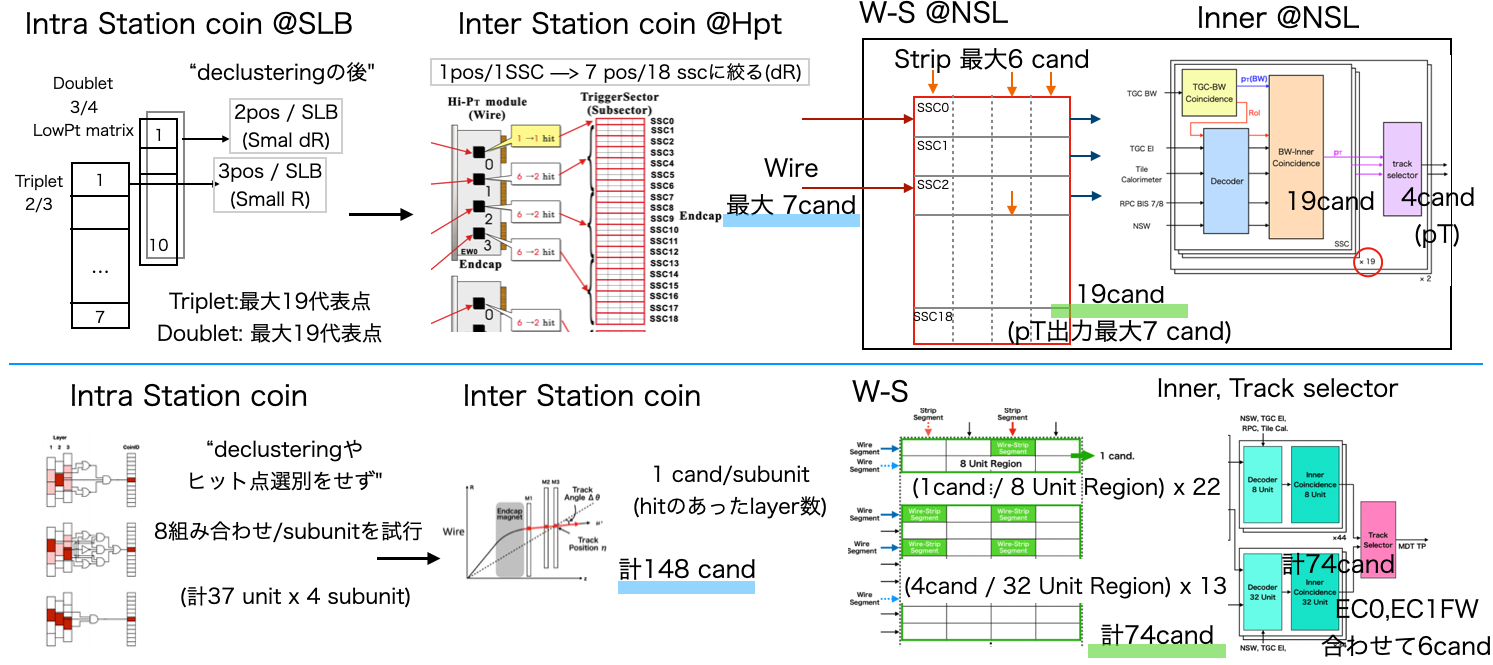
\includegraphics[width=16cm]{fig/SL/Trigger_Compare.png}
\caption[Run3と高輝度LHCのミューオン候補数の比較]{Run3と高輝度LHCのミューオン候補数の比較}
\label{SL_Trigger_Compare}
\end{figure}

また、L0 trigger latencyも2.5 $\mu$sから10 $\mu$sに拡張されたことにより、トリガー判定に使える時間にはまだ十分な余裕がある。図\ref{Trigger_latency_memo}に現状のトリガーロジックのトリガーレイテンシーを示す。陽子バンチ交差を時間の原点にとると、1120 ns後にはWire Strip Coincidenceは完了する。一方、NSWやTile カロリメーターからのトリガー情報がSLに到着するのは1425 ns後であり、この間の300 nsは現状有効活用されていない。

\begin{figure} 
\centering
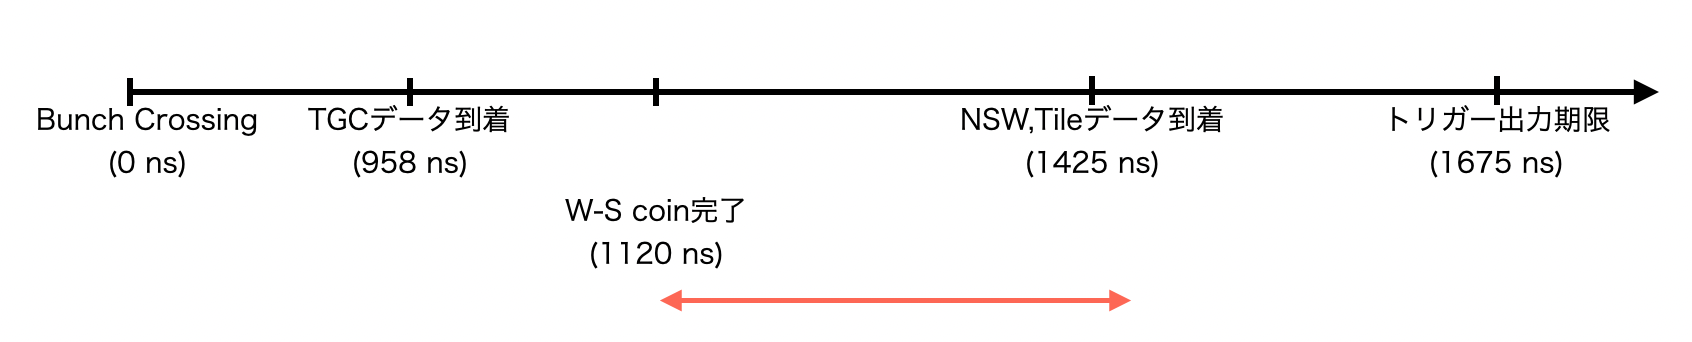
\includegraphics[width=16cm]{fig/SL/Trigger_latency_memo.png}
\caption[トリガーロジックのレイテンシー]{Cトリガーロジックのレイテンシー}
\label{Trigger_latency_memo}
\end{figure}

この2つのことから、Wire Strip Coincidence直後にInner Coincidenceに渡すミューオン候補を絞り込むロジックを挟む最適化を行うことで、トリガー性能を維持したまま、タイミング制約を大幅に緩和できると考えられる。仮にWire Strip Coincidenceから出力されるミューオン候補数を74 個から10個に絞りこんだとすると、SLRをまたぐ信号線は約85 \%程度削減することができる。またInner Coincidenceに並列に実装するロジックの数もこれに合わせて削減することができる。さらに、これに付随してInner Coincidenceから出力されるミューオン候補も自動的に削減されるため、Track Selectorの規模縮小にもつながる。

今後、Inner Coincidenceまでにミューオン候補をどれだけ削減するか、や何を基準に選択するか、などの詳細を決定するためのシミュレーション研究を専攻して進めていく予定である。